
\chapter{声波半空间无相位数据成像问题}

在本章中,我们基于半空间逆时偏移算法,针对半空间均匀介质障碍物成像问题提出了一种新的直接成像算法。该算法仅利用声波总场的模作为数据,不需要知道关于障碍物的先验信息,例如障碍物是否可穿透以及不可穿透障碍物的边界类型, 就可以确定嵌入在介质中障碍物的位置和形状。然后我们通过严格的分辨率分析,证明了该算法可以达到和原有算法相同的精度。最后,大量的数值算例验证了新算法对障碍物成像问题的有效性和抗干扰性。
\section{问题介绍}
我们以可穿透障碍物成像问题为例来介绍我们的算法,假设可穿透障碍物 $D\in\R^2_+=\{(x_1,x_2)^T:x_1\in\R,x_2>0\}$ 是一个有界的
Lipschitz 区域,其边界记为 $\Gamma_D$. 假设入射场 $u^i(x,x_s)$由位于半空间边界上的点源 $x_s$ 激发生成,其中 $x_s\in\Gamma_0=\{(x_1,x_2)^T:x_1\in\R,x_2=0\}$. 总场 $u(x,x_s)$ 为如下半空间障碍物问题的散射解:
\begin{eqnarray}
 \Delta u+k^2n(x)u=-\delta_{x_s}(x)\ \ in\ \ \R^2_+,\label{penetrable1}\\
 \frac{\partial u}{\partial x_2}=0\ \ on\ \ \Gamma_0,\\
 \sqrt{r}\left(\frac{\partial u}{\partial r}-\ii ku\right)\rightarrow0\ \ as\ \ r\rightarrow\infty,\ \ r=|x|,\label{Sommerfeld}
\end{eqnarray}
其中 $k>0$ 为波数,$n(x)\in L^{\infty}(\R^2_+)$ 是一个正的标量函数,且当$x\in\R^2_+\backslash D$时,$n(x)\equiv1$,
$\delta_{x_s}(\cdot)$是位于$x_s$处的点源。散射条件$(\ref{Sommerfeld})$即众所周知的Sommerfeld散射条件,它保证了
该散射问题的唯一性。在本章中,我们提到散射问题或散射解都是指满足Sommerfeld散射条件$(\ref{Sommerfeld})$。

令$N_k(x,y)$为半空间Hemholtz方程的Neumann格林函数:
\begin{equation}\label{Green}
  N_k(x,y)=\Phi_k(x,y)+\Phi_k(x,y'),
\end{equation}
其中$\Phi_k(x,y)=\frac{\ii}{4}H_0^{(1)}(k|x-y|)$是波数为$k$的Hemholtz方程基本解,$y'=(y_1,-y_2)$ 是 $y=(y_1,y_2)\in\R^2_+$关于边界$\Gamma_0$的镜像点。则
\eqref{penetrable1}-\eqref{Sommerfeld}可以理解为$u(x,x_s)=N_k(x,x_s)+u^s(x,x_s)$, 其中$u^s(x,x_s)$是如下问题的散射解
\begin{eqnarray}
  \Delta u^s(x,x_s)+k^2n(x)u^s(x,x_s)=-k^2(n(x)-1)N_k(x,x_s)\ \ in\ \ \R^2_+,\label{equ1}\\
  \frac{\partial u^s}{\partial x_2}(x,x_s)=0\ \ on\ \ \Gamma_0\label{equ2}.
\end{eqnarray}

在光栅衍射成像以及雷达散射成像问题中\cite{d89, dbc},相对于测量相位信息,对总场的模的测量更加易于处理,且经济有效。在求解无相位数据反散射问题中,有两种类型常用的方法。第一种方法是采用一些快速有效的相位恢复算法从无相位数据中提取或模拟出数据的相位信息,然后再将处理
后的数据输入到传统的成像算法来求解,详见文献\cite{fda, bv, nmp}。第二种方法是把问题化为一个最小二乘的优化模型,利用传统的迭代法来求解,其目的是最小化测量到的无相位数据与通过模型模拟生成的数据之间的误差,详见文献\cite{kr, LK2010, LK2011,bll,cmp}。

逆时偏移算法现如今在地球物理反问题中已经成为一种标准的成像处理技术,详见文献\cite{bcs}。它的主要思想是首先将在半空间边界接收到的散射场数据反传到背景介质当中,然后计算入射场和反传播场的互相关,最后得到我们想要的成像函数。在文献
\cite{cch_a,cch_e,ch_e}中,Zhiming Chen等人分别针对声波、电磁波和弹性波障碍物成像问题,从数学角度提出了相应的单频逆时偏移算法。并且,他们基于Hemholtz-Kirchhoff恒等式,对单频逆时偏移算法构建了严格的分辨率分析,为全空间逆时偏移算法建立了完备的数学理论基础。值得一提的是,文献\cite{cch_a,cch_e,ch_e}中的分析不需要几何光学近似或者高频渐进假设,而且他们证明了逆时偏移算法得到的成像函数实际上是以基本解的虚部$\Im\Phi_k(x,y)$作为入射场得到的散射问题解的远场模式。这表明成像函数将在散射体的边界聚焦,其分辨率即是光学衍射极限。

在文献\cite{ch_pha}中,Zhiming Chen等人针对声波全空间障碍物成像问题,基于全空间逆时偏移算法,提出一种仅使用无相位数据进行直接成像的算法。并且通过对成像函数的分辨率分析,其证明了新的无相位成像算法可以达到和全空间声波逆时偏移算法\cite{cch_a}相同的成像效果。之后他们将该想法推广到了全空间电磁波障碍物成像问题\cite{ch_e}。
为了进一步确定嵌入在一般半空间中障碍物的位置、大小和形状,他们在文献\cite{ch_ha}中,提出了求解一般声波半空间障碍物逆散射问题的逆时偏移算法,并在合理假设下构建了分辨率分析理论。值得一提的是,文献\cite{ch_ha}中的成像函数可以看做在应用地球物理反问题领域中,时域成像函数在频率域上的表现形式,详见文献Yu Zhang\cite{zs07, zs09} 。

文献\cite{ch_ha}主要是为解决问题\ref{ques_half}中的第一部分,其所提的半空间逆时偏移算法需要散射场的全部信息。为解决问题\ref{ques_half}中的第二部分,在本章中我们提出了一种半空间无相位数据成像算法,该算法仅需要使用总场数据的振幅信息即可。令 $\Omega$ 表示采样区域,以及$h=dist(\Omega,\Gamma_0)$. 我们一般假设所要寻找的障碍物$D$位于采样区域$\Omega$ 当中。令$\Gamma_0^d=\{(x_1,x_2)^T;x_1\in(-d,d),x_2=0\}$, 其中$d>0$表示孔穴。我们的源点$x_s$和接收点$x_r$将位于$\Gamma_0^d$ 上,孔穴$d$表明了源点及接收点的范围。令$u^i(x,x_s)=N_k(x,x_s)$,则文献中提出的逆时偏移成像函数如下,
\begin{equation}\label{IFullspace}
 \quad I_{\rm RTM}(z)=\Im\int_{\Gamma_{0}^d}\int_{\Gamma_0^d}\frac{\partial\Phi_k(x_s,z)}{\partial x_2(x_s)}\frac{\partial\Phi_k(x_r,z)}{\partial x_2(x_r)}
  \overline{u^s(x_r,x_s)}ds(x_r)ds(x_s),\  \  \forall z\in\Omega.\hspace{1.2cm}
\end{equation}
文献\cite{ch_ha}通过成像函数的分辨率分析,说明了该成像函数总是在散射体的边界聚焦。

在本章中,我们受文献\cite{ch_pha}启发,提出了一种新的直接成像算法,该算法仅需要总场数据的模作为数据。具体表示如下,
\begin{equation}\label{IPhaseless}
\quad  I^{\rm Phaseless}_{\rm RTM}(z)=\Im\int_{\Gamma_{0}^d}\int_{\Gamma_0^d}\frac{\partial\Phi_k(x_s,z)}{\partial x_2(x_s)}\frac{\partial\Phi_k(x_r,z)}{\partial x_2(x_r)}
  \Delta(x_r,x_s)ds(x_r)ds(x_s),\  \  \forall z\in\Omega.\hspace{0.6cm}
\end{equation}
其中
 \begin{equation}
   \Delta(x_r,x_s)=\frac{|u(x_r,x_s)|^2-|u^i(x_r,x_s)|^2}{u^i(x_r,x_s)}.
 \end{equation}
我们将在定理4.1中证明如下结果,
\begin{equation}
  I^{\rm Phaseless}_{\rm RTM}(z)=I_{\rm RTM}(z)+O\left(\frac{1}{\sqrt{kh}}\right),\  \  \forall z\in\Omega.
\end{equation}
该结果表明,如果源点和接收点的位置远离障碍物,我们提出的算法可以达到和原有算法相同的分辨率效果。

本章结构安排如下。在第二小节,我们将介绍所提出的新的半空间无相位数据直接成像算法。在第三小节,我们回顾一下已有的结论和文献\cite{ch_ha}中算法的分辨率分析,以便于比较。在第四小节,我们以可穿透障碍物逆散射问题为例考虑算法的分辨率分析。在第五小节,我们将理论分析结果推广到不可穿透障碍物逆散射问题。最后在第六小节,我们通过一些数值例子来验证算法的有效性和鲁棒性。
\section{半空间无相位逆时偏移算法}
在本小节,我们将介绍半空间无相位逆时偏移算法。假设在$\Gamma_0^d$上均匀分布着$N_s$个源点和$N_r$个接收点,其中$\Gamma_0^d=\{(x_1,x_2)^T;x_1\in(-d,d),x_2=0\}$, $d>0$表示孔穴。我们总是假设$D\subset\Omega$,其中$\Omega$为采样区域。

令$u^i(x,x_s)=N_k(x,x_s)$为源点处于$x_s\in\Gamma_0^d$的入射场, $|u(x_r,x_s)|=|u^s(x_r,x_s)+u^i(x_r,x_s)|$ 为我们在
接收点$x_r$出采集的无相位总场数据。其中$u^s(\cdot,x_s)$为问题 \eqref{equ1}-\eqref{equ2}的散射解。为了避免入射场$u^i(x,x_s)$ 在 $x=x_r$处的奇性, 我们总是假设 $x_s\neq x_r$, $s=1$,$\ldots$,$N_s$, $r=1$,$\ldots$,$N_r$。这个假设在实际应用中很容易满足。

半空间无相位逆时偏移算法的基本思想如下:第一步使用$\frac{\partial\Phi_k(x_r,z)}{\partial x_2(x_r)}$将修改过的数据
$ \Delta(x_r,x_s)$ 反传播到采样区域当中,第二步是计算$\frac{\partial\Phi_k(x_s,z)}{\partial x_2(x_s)}$ 和反传波场的互相关关系。

\begin{algorithm}[半空间无相位逆时偏移算法]\label{alg_phaseless}
设$|u(x_r,x_s)|=|u^s(x_r,x_s)+u^i(x_r,x_s)|$ 为我们在接收点$x_r\in\Gamma_0^d$出采集的无相位总场数据,其源点为$x_s\in\Gamma_0^d$.\\
$1^\circ$ 反传播: 对于 $s=1,\ldots,N_s$, 计算反传波场
\begin{equation}
  v_b(z,x_s)=\frac{|\Gamma_0^d|}{N_r}\sum\limits_{r=1}^{N_r}\frac{\partial\Phi_k(x_r,z)}{\partial x_2(x_r)}\Delta(x_r,x_s),\  \  \forall z\in\Omega.
\end{equation}
$2^\circ$ 互相关: 对于 $z\in\Omega$, 计算成像函数
\begin{equation}
  I_d(z)=\Im\left\{\frac{|\Gamma_0^d|}{N_s}\sum\limits_{s=1}^{N_s}\frac{\partial\Phi_k(x_s,z)}{\partial x_2(x_s)}v_b(z,x_s)
  \right\}.
\end{equation}
将反传波场$v_b(z,x_s)$代入到成像函数$I_d(z)$,可得
\begin{equation}
  \qquad I_d(z)=\Im\left\{\frac{|\Gamma_0^d||\Gamma_0^d|}{N_sN_r}
  \sum\limits_{s=1}^{N_s}\sum\limits_{r=1}^{N_r}
  \frac{\partial\Phi_k(x_s,z)}{\partial x_2(x_s)}\frac{\partial\Phi_k(x_r,z)}{\partial x_2(x_r)}
  \Delta(x_r,x_s)
  \right\},\  \ \forall z\in\Omega.\quad\quad
\end{equation}
\end{algorithm}
此公式将在本章所有数值算例中使用。若令$N_s,N_r\rightarrow\infty$,则上式可看做对如下积分的近似。
\begin{equation*}
 \qquad  I^{\rm Phaseless}_{\rm RTM}(z)=\Im\int_{\Gamma_0^d}\int_{\Gamma_0^d}\frac{\partial\Phi_k(x_s,z)}{\partial x_2(x_s)}\frac{\partial\Phi_k(x_r,z)}{\partial x_2(x_r)}
  \Delta(x_r,x_s)ds(x_r)ds(x_s),\  \  \forall z\in\Omega.\quad\quad
\end{equation*}

在第四小节进行分辨率分析时,我们将说明该积分是绝对收敛的。
\section{预备知识}
我们首先引入一些记号。对任意有界区域$U\subset\R^2$,令
\begin{equation*}
\|u\|_{H^1(U)}=
(\|\nabla\phi\|_{L^2(U)}^2+d_U^{-2}\|\phi\|^2_{L^2(U)})^{1/2}
\end{equation*}
为加权的$H^1(U)$范数,其中$d_U$表示$U$的直径。对半空间可穿透障碍物散射问题,仿照文献 \cite[Theorem 5.26]{cc14},我们可以建立如下的稳定的估计。
\begin{lemma}[稳定性估计]\label{lem:3.1}
令 $1-n(x)\in L^{\infty}(D)$, $g\in L^2(D)$ 分别是支集在 $D$ 上的标量函数, 则如下半空间Hemholtz散射问题
\begin{equation}\label{forward}
  \Delta w+k^2n(x)w=k^2(1-n(x))g\  \ in\  \ \R^2_+, \  \ \frac{\partial w}{\partial x_2}=0\  \  on\  \  \Gamma_0,
\end{equation}
存在唯一散射解 $w\in H^1(D)$. 更进一步,存在常数 $C>0$, 使得
\begin{equation}
    \|w\|_{H^1(D)}\leq C\|n\|_{L^{\infty}(D)}\|g\|_{L^2(D)}.
\end{equation}
\end{lemma}
由引理\ref{lem:3.1},我们可以定义解算子$\mathbb{S}:L^2(D)\rightarrow H^1(D)$,
\begin{equation*}
  w=\mathbb{S} g
\end{equation*}
其中散射场$w\in H^1(D)$ 为对应于入射场$g\in L^2(D)$的解。在本章中我们将以$\|\mathbb{S}\|$来表示$\mathbb{S}$的算子范数,
由引理\ref{lem:3.1}可知,其仅依赖于$k,n(x)$以及区域$D$。
对任意的$y,z\in\Omega$,定义
\begin{equation*}
    F(z,y)=-\frac{\ii}{2\pi}\int_0^{\pi}e^{\i k(z_1-y_1)\cos\theta+\i k(z_2-y_2)\sin\theta}d\theta.
\end{equation*}
显然我们有当$z=y$时,$F(z,y)=-\frac{\i}{2}$,并且根据文献\cite[Lemma 3.3]{ch_ha}可知,存在某个与$k$无关的常数$C$使得,
\begin{equation}\label{a1}
|F(z,y)|\leq C[(k|z-y|)^{-1/2}+(k|z-y|)^{-1}],\ \ \forall z,y\in\Omega.
\end{equation}
因此,$F(z,y)$具有和点扩散函数一样的性质:在$z=y$时,$-\Im F(z,y)$取得峰值;当$|z-y|$变大时,$-\Im F(z,y)$逐渐衰减。更进一步,根据\cite[Theorem 5.2]{ch_ha},可知关于由$(\ref{IFullspace})$ 所定义的成像函数$I_{\rm RTM}(z)$ 的分辨率分析定理。
\begin{theorem}[$I_{\rm RTM}(z)$的分辨率分析]\label{thm:3.1}
对任意的 $z\in\Omega$, 令$\psi(y,z)$为如下问题的散射解 $$
\Delta_y\psi(y,z)+k^2n(y)\psi(y,z)=-k^2(n(y)-1)\overline{F(z,y)}\ \ in\ \ \R^2.$$
则我们有, 对任意的 $z\in\Omega$,$$
I_{\rm RTM}(z)=-\frac{1}{4}\Im\int_Dk^2(1-n(y))(\psi(y,z)+\overline{F(z,y)})\overline{F(z,y)}dy+W_{\hat{I}}(z),$$
其中 $\left|W_{\hat{I}}(z)\right|\leq C(1+kd_D)^4((kh)^{-1/2}+h/d)$,关于$z\in\Omega$一致成立。
\end{theorem}
\begin{remark}
对可穿透障碍物散射问题,$\psi(y,z)$即是以$\overline{F(z,y)}$做为入射场的散射解。根据\eqref{a1},我们期望成像函数$I_{\rm RTM}(z)$ 将总是在散射体边界上取得峰值,然后远离散射体时逐渐衰减。此外,文献\cite{ch_ha}以声软障碍物逆散射问题为例说明了,如果成像所使用的散射数据仅仅在$\Gamma_0$上采集,则不可能对散射体的下边界进行成像。并且他们在假设$kh\gg1$ 和 $d\gg h$ 成立时,采用稳项定理以及Kirchhoff 高频渐进逼近,结合散射系数给出了数学证明和物理解释。文献\cite{ch_ha}中大量的数值例子验证了成像函数$I_{\rm RTM}(z)$的有效性、实用性和抗干扰性。
\end{remark}
\section{无相位逆时偏移算法的分辨率分析}
在本小节,我们将说明新提出的无相位逆时偏移算法成像函数$I^{\rm phaseless}_{\rm RTM}(z)$可以达到和原有算法成像函数$I_{\rm RTM}(z)$ 相同的分辨率。我们将作出如下假设,
\begin{equation}\label{ass}
|y_1-z_1|\leq Ch,\ z_2\leq Ch,\ \ \forall y,z\in\Omega,\ \ \mbox{where }h=dist(\Omega,\Gamma_0).
\end{equation}
下面的定理是本章的主要结论。
\begin{theorem}[无相位逆时偏移算法的分辨率分析]\label{main}
 若$|u(x_r,x_s)|=|u^s(x_r,x_s)+u^i(x_r,x_s))|$为所测量的散射总场的无相位数据,其中 $u^s(x,x_s)$ 是\eqref{equ1}-\eqref{equ2} 以$u^i(x,x_s)=N_k(x,x_s)$ 为入射场的散射解,则我们有
\begin{equation*}
  I^{\rm phaseless}_{\rm RTM}(z)=I_{\rm RTM}(z)+ R^{\rm phaseless}_{\rm RTM}(z),\ \ \forall z\in\Omega,
\end{equation*}
其中
\begin{equation*}
\left| R^{\rm phaseless}_{\rm RTM}(z)\right|\leq C(1 + \|\mathbb{S}\|)^2(kh)^{-1/2},\ \ \forall z\in\Omega.
\end{equation*}
其中常数$C>0$ 可能依赖于 $kd_D$ 和 $\|n(\cdot)\|_{L^{\infty}(D)}$,但是与 $k,h,d_D$无关。
\end{theorem}
该定理的证明主要依赖于以下几个引理,我们首先观察到
\begin{equation*}
  \Delta(x_r,x_s)=\overline{u^s(x_r,x_s)}+\frac{|u^s(x_r,x_s)|^2}{u^i(x_r,x_s)}+\frac{u^s(x_r,x_s)
  \overline{u^i(x_r,x_s)}}{u^i(x_r,x_s)}.
\end{equation*}
据此可得
\begin{eqnarray*}\label{I123}
\begin{array}{lll}
 I^{\rm Phaseless}_{\rm RTM}(z)&=& \Im\int_{\Gamma_{0}^d}\int_{\Gamma_0^d}\frac{\partial\Phi_k(x_s,z)}{\partial x_2(x_s)}\frac{\partial\Phi_k(x_r,z)}{\partial x_2(x_r)}
  \overline{u^s(x_r,x_s)}  ds(x_r)ds(x_s)\\
  & &\\
  & &+ \Im\int_{\Gamma_{0}^d}\int_{\Gamma_0^d}\frac{\partial\Phi_k(x_s,z)}{\partial x_2(x_s)}\frac{\partial\Phi_k(x_r,z)}{\partial x_2(x_r)}\frac{|u^s(x_r,x_s)|^2}{u^i(x_r,x_s)}ds(x_r)ds(x_s)\\
  & &\\
  & & +\Im\int_{\Gamma_{0}^d}\int_{\Gamma_0^d}\frac{\partial\Phi_k(x_s,z)}{\partial x_2(x_s)}\frac{\partial\Phi_k(x_r,z)}{\partial x_2(x_r)}
  \frac{u^s(x_r,x_s)
  \overline{u^i(x_r,x_s)}}{u^i(x_r,x_s)}ds(x_r)ds(x_s)\\
  & &\\
  &:=& I_{\rm RTM}(z)+{\rm I}_2+{\rm I}_3
\end{array}
\end{eqnarray*}
我们的目标是说明当$kh\gg1$时,$I_2,I_3$是小量。首先,由文献\cite[(1.22)-(1.23)]{cg09}可得如下关于Hankel函数的估计。
\begin{lemma}\label{lem:4.0}
我们有
\begin{equation*}
  |H_0^{(1)}(t)|\leq\left(\frac{1}{\pi t}\right)^{\frac{1}{2}},\  \
  |H_1^{(1)}(t)|\leq\left(\frac{1}{\pi t}\right)^{\frac{1}{2}}+\frac{1}{\pi t},\  \ \forall t>0.
\end{equation*}
\end{lemma}
为了以后的说明,我们将使用如下记号,对任意的$x_s,x_r\in\R^2_+$,
\begin{equation*}
  x_s=(x_{1s},x_{2s}),\ \ x_r=(x_{1r},x_{2r})
\end{equation*}
\begin{lemma}\label{lem:4.1}
对任意的$x_s, x_r\in\Gamma_0^d$,我们有
\begin{equation*}
  |u^s(x_r,x_s)|\leq C(1 + \|\mathbb{S}\|)[kd(x_r,D)]^{-1/2}[kd(x_s,D)]^{-1/2},
\end{equation*}
其中 $d(x,D)=\min_{y\in \overline D}|x-y|$是 $x\in\Gamma^d_0$和 $D$之间的距离, 且常数 $C>0$可能依赖于 $kd_D, \|n(\cdot)\|_{L^{\infty}(D)}$,但与 $k, d_D$无关。
\end{lemma}
\debproof
由积分表示定理可知,
\begin{eqnarray*}
  u^s(x_r,x_s)=k^2\int_{D}[n(y)-1]N_k(x_r,y)[u^s(y,x_s)+N(y,x_s)]ds(y).
\end{eqnarray*}
则由引理\ref{lem:3.1}可知,
\begin{eqnarray*}
|u^s(x_r,x_s)|\leq Ck^2\|n\|_{L^\infty(D)}(1+\|\mathbb{S}\|)\|N_k(x_r,\cdot)\|_{L^2(D)}\|N_k(\cdot,x_s)\|_{L^2(D)}.
\end{eqnarray*}
由引理\ref{lem:4.0} ,我们有对任意的$x_r\in\Gamma_0^d,y\in D$,
\begin{equation*}
|N_k(x_r,y)|=2|\Phi_k(x_r,y)|\leq (k|x_r-y|)^{-1/2}
\leq [kd(x_r,D)]^{-1/2}
\end{equation*}
类似地,
\begin{equation*}
  |N_k(y,x_s)|\leq [kd(x_s,D)]^{-1/2},\ \ \forall x_s\in\Gamma_0^d,y\in D
\end{equation*}
根据上面的估计可得,
\begin{equation*}
|u^s(x_r,x_s)|\leq C(kd_D)^2\|n\|_{L^\infty(D)}(1+\|\mathbb{S}\|)[kd(x_r,D)]^{-1/2}[kd(x_s,D)]^{-1/2}.
\end{equation*}
于是该引理得到证明。
\finproof
\begin{lemma}\label{lem:new}
令 $kh\geq 1$,记 $\Gamma_0^{(a,b)}=\{x\in\Gamma_0:x_1\in (a,b)\}$,其中 $a,b\in\R, a<b$。
则对 $\forall z\in\Omega$, 我们有
\begin{equation*}
\left|\int_{\Gamma_0^{(a,b)}}\frac{\partial\Phi_k(x,z)}{\partial x_2}f(x)ds(x)\right|\leq (kz_2)^{1/2}\|f\|_{L^\infty(\Gamma_0^{(a,b)})}.
\end{equation*}
\end{lemma}
\debproof
由于对$\forall x\in\Gamma_0^{(a,b)},z\in\Omega$, $k|x-z|\geq kh\ge 1$。 根据引理\ref{lem:4.0},我们有
\begin{equation}\label{b2}
\left|\frac{\partial\Phi_k(x,z)}{\partial x_2}\right|=\left|\frac{\i k}{4}H^{(1)}_1(k|x-z|)  \frac{z_2}{|x-z|}\right|\leq \frac 1{2\sqrt{\pi}}\frac{k^{1/2}z_2}{|x-z|^{3/2}}.
\end{equation}
然后做变换 $t=(x_1-z_1)/z_2$,可得
\begin{equation*}
\left|\int_{\Gamma_0^{(a,b)}}\frac{\partial\Phi_k(x,z)}{\partial x_2}f(x)ds(x)\right|\leq\frac{(kz_2)^{1/2}}{2\sqrt\pi}\|f\|_{L^\infty(\Gamma_0^{(a,b)})}\int^\infty_{-\infty}\frac 1{(1+t^2)^{3/2}}dt.
\end{equation*}
另一方面
\begin{equation*}
\int^\infty_{-\infty}\frac 1{(1+t^2)^{3/2}}dt\leq 2\left[1+\int^\infty_1\frac{t}{(1+t^2)^{3/2}}dt\right]=2(1+1/\sqrt 2)\leq 2\sqrt\pi.
\end{equation*}
于是该引理得到证明。
\finproof

现在我们可以给出(\ref{I123})中第二项$I_2$的估计。

\begin{lemma}\label{lem:4.3}
令 $kh\geq 1$, 则 $\forall z\in\Omega$,我们有
\begin{equation*}
|{\rm I}_2|\leq C(1 + \|\mathbb{S}\|)^2(kh)^{-1/2}
\end{equation*}
其中常数$C>0$ 可能依赖于 $kd_D,\|n(\cdot)\|_{L^{\infty}(D)}$,但是与$k,h,d_D$无关。
\end{lemma}
\debproof
令$\Omega_k=\{(x_r,x_s)\in \Gamma_0^d\times\Gamma_0^d: |x_r-x_s|\leq 1/(2k)\}$。根据\cite[Lemma 3.3]{ch_pha} 中的估计可知,
\begin{equation*}
    |H^{(1)}_0(k|x_r-x_s|)| \ge \frac 2{5\pi e}\ln(k|x_r-x_s)|\ge \frac{2\ln 2}{5\pi e},\ \ \forall (x_r,x_s)\in\Omega_k.
\end{equation*}
由于$\forall x\in\Gamma_0^d$, $d(x,D)\geq h$,则根据引理\ref{lem:4.1}可知
\begin{equation*}
 \left|
  \frac{u^s(x_r,x_s)^2}{u^i(x_r,x_s)}\right|\leq C(1+\|\mathbb{S}\|)^2(kh)^{-2},
\end{equation*}
从而由引理\ref{lem:new}可得
$$\label{I21}
\left|\int\hskip-6pt\int_{\Omega_k} \frac{\partial\Phi_k(x_s,z)}{\partial x_2(x_s)}\frac{\partial\Phi_k(x_r,z)}{\partial x_2(x_r)}
  \frac{|u^s(x_r,x_s)|^2}{u^i(x_r,x_s)}ds(x_r)d(x_s)\right|
\leq C(1+\|\mathbb{S})^2(kh)^{-1},
$$
其中我们使用了假设\eqref{ass}中的条件: $z_2\leq C h$,$\forall z\in\Omega$。

现在我们来估计在$\Gamma_0^d\times\Gamma_0^d\backslash\overline\Omega_k$上的积分。根据 \cite[p. 446]{watson} 可知,$t|H_{0}^{(1)}(t)|^2$ 在 $t >0$ 时是一个单调递增函数,则
\begin{equation*}
\forall (x_r,x_s)\in \Gamma_0^d\times\Gamma_0^d\backslash\overline\Omega_k,\ \ |x_r-x_s|\geq 1/(2k)
\end{equation*}
于是我们有
\begin{equation*}
|x_r-x_s||u^i(x_r,x_s)|^2\geq\frac{1}{32} k^{-1}\left|H_{0}^{(1)}\left(\frac 12\right)\right|^2=Ck^{-1}.
\end{equation*}
由于$|x_r-x_s|\leq d(x_r,D)+d(x_s,D)$以及当$ x\in\Gamma_0^d$时,$d(x,D)\geq h$,根据引理 \ref{lem:4.1}可得
\begin{equation*}
\left|\frac{u^s(x_r,x_s)^2}{u^i(x_r,x_s)}\right|\leq C(1+\|\mathbb{S}\|)^2\frac{k^{1/2}|x_r-x_s|^{1/2}}{k^2d(x_r,D)d(x_s,D)}\leq C(1+\|\mathbb{S})^2(kh)^{-3/2}.
\end{equation*}
于是有引理\ref{lem:new}可得
\begin{eqnarray*}\label{I22}
\begin{array}{lll}
& &\left|\int\hskip-6pt\int_{ \Gamma_0^d\times\Gamma_0^d\backslash\overline\Omega_k} \frac{\partial\Phi_k(x_s,z)}{\partial x_2(x_s)}\frac{\partial\Phi_k(x_r,z)}{\partial x_2(x_r)}
  \frac{|u^s(x_r,x_s)|^2}{u^i(x_r,x_s)}ds(x_r)d(x_s)\right|\\
& &\\
&\leq&C(1 + \|\mathbb{S}\|)^2(kh)^{-1/2}.
\end{array}
\end{eqnarray*}
由估计(\ref{I21})-(\ref{I22})可知,该引理得到证明。
\finproof
现在我们来估计(\ref{I123})中的第三项$I_3$。为估计此项,令$\delta=(h/k)^{\frac12}$,并定义集合$Q_\delta$如下:
\begin{equation}\label{Qdelta}
Q_\delta=\{(x_r,x_s)\in \Gamma_0^d\times\Gamma_0^d:\ |x_s-x_r|\leq \delta\}
\end{equation}
\begin{lemma}\label{lem:4.4}
我们有,对任意的$z\in\Omega$,
$$
\left|\int\hskip-6pt\int_{Q_{\delta}}\frac{\partial\Phi_k(x_s,z)}{\partial x_2(x_s)}\frac{\partial\Phi_k(x_r,z)}{\partial x_2(x_r)}
  \frac{u^s(x_r,x_s)
  \overline{u^i(x_r,x_s)}}{u^i(x_r,x_s)}ds(x_r)d(x_s)\right|\leq C(1 + \|\mathbb{S}\|)(kh)^{-1/2},
$$
其中常数 $C>0$可能依赖于$kd_D,\|n(\cdot)\|_{L^{\infty}(D)}$,但是与$k, h, d_D$无关。
\end{lemma}
\debproof
我们将被积区域$Q_{\delta}$分成几份,易得
\begin{eqnarray*}
\begin{array}{lll}
& &\int\hskip-6pt\int_{Q_{\delta}}\frac{\partial\Phi_k(x_s,z)}{\partial x_2(x_s)}\frac{\partial\Phi_k(x_r,z)}{\partial x_2(x_r)}
  \frac{u^s(x_r,x_s)
  \overline{u^i(x_r,x_s)}}{u^i(x_r,x_s)}ds(x_r)d(x_s) \\
& &\\
&=&\int^{-d+\delta}_{-d}\frac{\partial\Phi_k(x_s,z)}{\partial x_2(x_s)}\int^{x_{1s}+\delta}_{-d}
\frac{\partial\Phi_k(x_r,z)}{\partial x_2(x_r)}\frac{u^s(x_r,x_s)
  \overline{u^i(x_r,x_s)}}{u^i(x_r,x_s)}dx_{1r}dx_{1s}\\
& &\\
& &+\int^{d-\delta}_{-d+\delta}\frac{\partial\Phi_k(x_s,z)}{\partial x_2(x_s)}\int^{x_{1s}+\delta}_{x_{1s}-\delta}\frac{\partial\Phi_k(x_r,z)}{\partial x_2(x_r)}\frac{u^s(x_r,x_s)
  \overline{u^i(x_r,x_s)}}{u^i(x_r,x_s)}dx_{1r}dx_{1s}\\
& &\\
& &+\int^d_{d-\delta}\frac{\partial\Phi_k(x_s,z)}{\partial x_2(x_s)}\int^d_{x_{1s}-\delta}\frac{\partial\Phi_k(x_r,z)}{\partial x_2(x_r)}
  \frac{u^s(x_r,x_s)
  \overline{u^i(x_r,x_s)}}{u^i(x_r,x_s)}dx_{1r}dx_{1s}\\
  & &\\
&:=&{\rm II_1}+{\rm II_2}+{\rm II_3}.
\end{array}
\end{eqnarray*}
由于当$x_s\in\Gamma_0^d$时,$|x_s-z|\geq z_2$,从而根据 \eqref{b2}、 引理 \ref{lem:4.1}和引理\ref{lem:new}可知
$$
|{\rm II}_1|\leq\delta\cdot\frac{k^{1/2}z_2}{z_2^{3/2}}\cdot (kz_2)^{1/2}\cdot C(1+\|\mathbb{S}\|)(kh)^{-1}\leq C(1+\|\mathbb{S}\|)(kh)^{-1/2}.
$$
其中我们用到了定义$\delta=(h/k)^{1/2}$。其余两项的估计类似,于是该引理得到证明。

\finproof
为了估计在$\Gamma_0^d\times \Gamma_0^d\backslash \overline Q_\delta$上的积分,我们首先回顾下文献中关于振荡积分的
Van der Corput引理,详见文献\cite[P.152]{grafakos}和\cite[Lemma 3.2]{ch_ha}。
\begin{lemma}\label{lem:4.2}
假设$-\infty<a<b<\infty$, $\lambda>0$以及$u$ 是定义在 $(a,b)$上的$C^2$函数。 若当 $t\in (a,b)$时,$|u'(t)|\geq 1$;并且
$u'$ 在$(a,b)$上单调。 则对任意定义在$(a,b)$的满足一阶导数可积的函数$\phi$,可使得如下不等式成立:
\begin{equation*}
\left|\int^b_a \phi(t)e^{\i\lambda u(t)}dt\right|\leq 3\lambda^{-1}\left[|\phi(b)|+\int^b_a|\phi'(t)|dt\right].
\end{equation*}
\end{lemma}
\begin{lemma}\label{lem:4.5}
对任意的$a,b\in\R, a<b$, 可以证明
$$
    \left|\int_{\Gamma_0^{(a,b)}} \frac{\partial\Phi_k(x,z)}{\partial x_2} \Phi_k(x,y) e^{-2\i k x_{1}} ds(x)\right|\leq C (kh)^{-1}, \quad \forall y,z \in \Omega,
$$
其中$C$ 可能依赖于 $kd_D, \|n(\cdot)\|_{L^{\infty}(D)}$,但是与 $k, h, d_D,a,b$无关。
\end{lemma}
 \debproof
由\ref{lem:4.0}以及文献\cite[P.197]{watson}中关于Hankel函数的渐进估计可知,对于$n=1,2$,
\begin{equation}\label{Hankel}
  H^{(1)}_n(t)=\left(\frac{2}{\pi t}\right)^{\frac{1}{2}}e^{\ii(t-\frac{n\pi}{2}-\frac{\pi}{2})}+R_n(t),\  \ |R_n(t)|\leq Ct^{-\frac{3}{2}},\  \ \forall t>0,
\end{equation}
据此可得,
$$
	\frac{\partial\Phi_k(x,z)}{\partial x_2} \Phi_k(x,y) = -\frac{1}{8\pi}\frac{z_2}{|x-z|^2} e^{\ii k (|x-z|+|x-y|)} + R(x,y,z),
$$
其中
$$
\begin{array}{lll}
|R(x,y,z)|&\leq&Ck^{-1}|x-z|^{-1/2}|x-y|^{-3/2}+Ck^{-1}|x-z|^{-3/2}|x-y|^{-1/2}\\
& &\\
& &+\ Ck^{-2}|x-z|^{-3/2}|x-y|^{-3/2}.
\end{array}
$$
直接带入上式进行估计可得,
\begin{equation}\label{c0}
\left|\int_{\Gamma_0^{(a,b)}} R(x,y,z) e^{-2\ii k x_{1}} ds(x)\right|\leq C (kh)^{-1}.
\end{equation}
故而我们只需估计如下积分即可。
\begin{equation*}
{\rm III}=\int_{\Gamma_0^{(a,b)}} \frac{z_2}{|x-z|^2} e^{\ii k (|x-z|+|x-y|-2x_{1})} ds(x).
\end{equation*}
做如下变量替换$t=(x_{1}-z_1)/z_2$,然后可得,
\begin{equation*}
{\rm III}=e^{-2\ii kz_1}\int^{b'}_{a'}\frac{1}{1+t^2}\,e^{\ii kz_2v(t)}dt,
\end{equation*}
其中 $b'=(b-z_1)/z_2,a'=(a-z_1)/z_2$,以及
\begin{equation*}
v(t)=\sqrt{1+t^2}+\sqrt{(t+t_1)^2+t_2^2}-2t,\ \ t_1=\frac{x_1-z_1}{z_2},t_2=\frac{x_2}{z_2}.
\end{equation*}
直接计算可知,
$$
v'(t)=\frac{t}{\sqrt{1+t^2}}+\frac{t+t_1}{\sqrt{(t+t_1)^2+t_2^2}}-2,\ \
v''(t)=\frac{1}{(1+t^2)^{3/2}}+\frac{t^2_2}{[(t+t_1)^2+t_2^2]^{3/2}}.
$$
令 $t_0=\max(0,-t_1)$, 则当$t\leq t_0$时有$v'(t)\leq -1$。于是根据\ref{lem:4.2},可得
\begin{equation}\label{c1}
\left|\int_{a'}^{\min(t_0,b')}\frac{1}{1+t^2}\,e^{\ii kz_2v(t)}\right|\leq C(kh)^{-1}.
\end{equation}
若$t_0\geq b'$,则根据\eqref{c0}和 \eqref{c1}即可完成该引理的证明。 否则,我们不妨设 $t_0<b'$,然后分部积分可得下式,
$$
\int^{b'}_{t_0}\frac 1{1+t^2}e^{\i kz_2v(t)}dt=\left[\frac{e^{\ii kz_2v(t)}}{\ii kz_2(1+t^2)v'(t)}\right]^{b'}_{t_0}-\int^{b'}_{t_0}\frac{-2tv'(t)-(1+t^2)v''(t)}
{\ii kz_2(1+t^2)^2v'(t)^2}dt.
$$
由$v'(t)\leq -1+t/\sqrt{1+t^2}$,可知对$\forall t\geq 0$,$(1+t^2)v'(t)\leq -1/2$。于是根据Van der Corput 引理可得,
\begin{equation}\label{c2}
\left|\int^{b'}_{t_0}\frac 1{1+t^2}e^{\i kz_2v(t)}dt\right|\le C(kh)^{-1}+C(kh)^{-1}\int^{b'}_{t_0}|2tv'(t)+(1+t^2)v''(t)|dt.
\end{equation}
现在为我们令$v=v_1+v_2$,其中
\begin{equation*}
v_1(t)=\sqrt{1+t^2}-t,\ \ v_2(t)=\sqrt{(t+t_1)^2+t_2^2}-t.
\end{equation*}
记$\Delta=[(t+t_1)^2+t_2^2]^{1/2}$,直接计算可得
\begin{equation*}
2tv_2'(t)+(1+t^2)v_2''(t)=\frac{t^2_2\,[-2t\Delta^2+(1+t^2)(t+t_1+\Delta)]}{\Delta^3[t+t_1+\Delta]}.
\end{equation*}
观察到对$t\geq t_0$, $t+t_1\geq0$,由\eqref{ass}可知 $|t_1|\leq C$,进而可得
\begin{equation*}
 |2tv_2'(t)+(1+t^2)v_2''(t)|\leq Ct^2/\Delta^4\leq C\Delta^{-2},
\end{equation*}
类似地,可以证明
\begin{equation*}
  |2tv_1'(t)+(1+t^2)v_1''(t)|\le C(1+t^2)^{-1}
\end{equation*}
进一步,由于$\Delta\geq|t_2|\geq C$, 积分 \eqref{c2}是有界的。故而下式成立
\begin{equation}\label{c3}
 \left|\int^{b'}_{t_0}\frac 1{1+t^2}e^{\i kz_2v(t)}dt\right|\le C(kh)^{-1}.
\end{equation}
结合上式以及\eqref{c0}-\eqref{c1},则该引理得到证明。
\finproof
\begin{lemma}\label{lem:4.6}
令 $a,b\in\R, a<b$,则 $\forall x_r\in\Gamma_0^d,z\in\Omega$,
\begin{eqnarray*}
    \left|\int_{\Gamma_0^{(a,b)}}\frac{\partial\Phi_k(x_s,z)}{\partial x_2(x_s)} u^s(x_r,x_s) e^{-2\ii k x_{1s}} ds(x_s)\right|\leq C(1 + \|\mathbb{S}\|) (kh)^{-1},\\
    \left|\int_{\Gamma_0^{(a,b)}}\frac{\partial\Phi_k(x_r,z)}{\partial x_2(x_r)} u^s(x_r,x_s) e^{-2\ii k x_{1r}} ds(x_r)\right|\leq C(1 + \|\mathbb{S}\|) (kh)^{-1},
\end{eqnarray*}
其中$C$可能依赖于$kd_D,\|n(\cdot)\|_{L^{\infty}(D)}$,但是与$k, h, d_D,a,b$无关。
\end{lemma}

\debproof 由于两者类似,我们以第一个不等式的证明为例。
定义$w(y,z)$是散射场$u^s(\cdot,x_s)$关于源点$x_s$在$\Gamma_0^{(a,b)}$上的线性组合,
\begin{equation}
    w(y,z) =\int_{\Gamma_0^{(a,b)}} \frac{\partial\Phi_k(x_s,z)}{\partial x_2(x_s)} u^s(y,x_s) e^{-2\ii k x_{1s}} ds(x_s),\ \ \forall y\in\R^2_+,
\end{equation}
则$w(y,z)$是以$g(y,z)$为入射场的问题 (\ref{forward})的散射解,其中
\begin{equation*}
    g(y,z)= \int_{\Gamma_0^{(a,b)}} \frac{\partial\Phi_k(x_s,z)}{\partial x_2(x_s)} N_k(y,x_s) e^{-2\ii k x_{1s}} ds(x_s).
\end{equation*}
根据引理\ref{lem:4.5}可知, $|g(y,z)|\leq C (kh)^{-1}$。进一步由积分表示定理,
\begin{equation*}
w(x_r,z)=k^2\int_{D}[n(y)-1]N_k(x_r,y)[w(y,z)+g(y,z)]ds(y).	
\end{equation*}
于是由引理\ref{lem:3.1}可得
$$
\begin{array}{lll}
|w(x_r,z)|&\leq&k^2\|n(\cdot)\|_{L^\infty(D)}\|N_k(x_r,\cdot)\|_{L^2(D)}(\|\mathbb{S}\|\|g(\cdot,z)\|_{L^2(D)}+\|g(\cdot,z)\|_{L^2(D)})\\
& &\\
&\leq&C(1+\|\mathbb{S}\|)(kh)^{-1}.
\end{array}
$$
则该引理得到证明。
\finproof
\begin{lemma}\label{lem:4.7}
对任意的$z\in\Omega$,
\begin{eqnarray*}
& &\left|\int\hskip-6pt\int_{\Gamma_0^d\times \Gamma_0^d\backslash \overline Q_\delta}\frac{\partial\Phi_k(x_s,z)}{\partial x_2(x_s)}\frac{\partial\Phi_k(x_r,z)}{\partial x_2(x_r)}\frac{u^s(x_r,x_s)
  \overline{u^i(x_r,x_s)}}{u^i(x_r,x_s)}ds(x_r)d(x_s)\right|\\
  &\leq& C(1+\|\mathbb{S}\|)(kh)^{-1/2}.
\end{eqnarray*}
其中$C$可能依赖于$kd_D,\|n(\cdot)\|_{L^{\infty}(D)}$,但是与$k, h, d_D,a,b$无关。
\end{lemma}
\debproof
由定义$u^i(x_r,x_s)=2\Phi(x_r,x_s)$,根据Hankel函数的渐进估计 \eqref{Hankel},可得
\begin{eqnarray*}
  \frac{\overline{u^i(x_r,x_s)}}{u^i(x_r,x_s)}=-e^{-2\ii k|x_r-x_s|+\ii\frac{\pi}{2}}+\rho_0(x_r,x_s),\  \  |\rho_0(x_r,x_s)|\leq C(k|x_r-x_s|)^{-1}.
\end{eqnarray*}
由于当$x_r,x_s\in\Gamma_0^d\times\Gamma_o^d\backslash\overline Q_\delta$时,$k|x_r-x_s|\geq C\sqrt{kh}$。 于是由引理 \ref{lem:4.1}和\ref{lem:new}可得
\begin{eqnarray}\label{d1}
& &\left|\int\hskip-6pt\int_{\Gamma_0^d\times \Gamma_0^d\backslash \overline Q_\delta}\frac{\partial\Phi_k(x_s,z)}{\partial x_2(x_s)}\frac{\partial\Phi_k(x_r,z)}{\partial x_2(x_r)}
  u^s(x_r,x_s)\rho_0(x_r,x_s)
  ds(x_r)d(x_s)\right| \nonumber\\
  &\leq&C(1+\|\mathbb{S}\|)(kh)^{-\frac{1}{2}}.
\end{eqnarray}
现在我们只需估计如下积分,
\begin{eqnarray}
& &\int\hskip-6pt\int_{\Gamma_0^d\times \Gamma_0^d\backslash \overline Q_\delta}
\frac{\partial\Phi_k(x_r,z)}{\partial x_2(x_r)}\frac{\partial\Phi_k(x_s,z)}
{\partial x_2(x_s)}u^s(x_r,x_s) e^{-2\ii k |x_r-x_s|} ds(x_r)ds(x_s)\nonumber\\
&=&\int_{-d}^{d-\delta} \frac{\partial\Phi_k(x_r,z)}{\partial x_2(x_r)}\left[\int_{x_{1r}+\delta}^{d} \frac{\partial\Phi_k(x_s,z)}{\partial x_2(x_s)}u^s(x_r,x_s) e^{-2\ii k (x_{1s}-x_{1r})} dx_{1s}\right] dx_{1r}\nonumber\\
& &+\int_{-d}^{d-\delta} \frac{\partial\Phi_k(x_s,z)}{\partial x_2(x_s)}
\left[\int_{x_{1s}+\delta}^{d} \frac{\partial\Phi_k(x_r,z)}{\partial x_2(x_r)}u^s(x_r,x_s) e^{-2\ii k (x_{1r}-x_{1s})}
dx_{1r}\right] dx_{1s}\nonumber\\
&:=&{\rm IV}_1+{\rm IV}_2.\label{d2}
\end{eqnarray}
根据引理\ref{lem:4.6}可得,
\begin{eqnarray}
	 \qquad \left|\int_{x_{1r}+\delta}^{d} \frac{\partial\Phi_k(x_s,z)}{\partial x_2(x_s)}u^s(x_r,x_s) e^{-2\i kx_{1s}} dx_{1s} \right|\leq C(1+\|\mathbb{S}\|)(kh)^{-1}.
\end{eqnarray}
由引理\ref{lem:new}可知$|{\rm IV}_1|\leq C(1+\|\mathbb{S}\|)(kh)^{-1/2}$。 类似地,我们可以证明$|{\rm IV}_2|\leq C(1+\|\mathbb{S}\|)(kh)^{-1/2}$。
于是该引理得到证明。
\finproof

现在我们可以来完成本章主要定理的证明。

{\bf 定理\ref{main}的证明}: 由 \eqref{I123}可知,定理\ref{main}为引理\ref{lem:4.3},引理\ref{lem:4.4}和引理
\ref{lem:4.7}联合起来的直接推论。
$\Box$
\section{不可穿透情形}
在本小节我们考虑如何使用新提出的半空间无相位逆时偏移算法算法来确定不可穿透障碍物的位置和形状,例如声软障碍物和具有阻抗边界的障碍物。

对于声软障碍物,测量数据为总场的无相位数据$|u(x_r,x_s)|=
|u^s(x_r,x_s)+N_k(x_r,x_s)|$,其中$u^s(x_r,x_s)$为如下问题的散射解,
\begin{eqnarray}
 \Delta u^s+k^2u^s=0,&in& \R^2_+\backslash\overline{D},\label{sound-soft1}\\
  u^s(x,x_s)=-N_kx,x_s),&on& \Gamma_D,\label{sound-soft2}\\
  \frac{\partial u^s}{\partial x_2}(x,x_s)=0,&on& \Gamma_0\label{sound-soft3}.
\end{eqnarray}
通过对第四节中的证明做一些简单的修改,我们可以证明如下定理。
\begin{theorem}\label{thm:5.1}
若测量数据为总场的无相位数据$|u(x_r,x_s)|=|u^s(x_r,x_s)+N_k(x_r,x_s)|$, 其中$u^s(x_r,x_s)$为满足问题$(\ref{sound-soft1})
-(\ref{sound-soft3})$的散射解,则
\begin{equation*}
  I^{\rm phaseless}_{\rm RTM}(z)=I_{\rm RTM}(z)+ R^{\rm phaseless}_{\rm RTM}(z),\ \ \forall z\in\Omega,
\end{equation*}
其中 $$\left| R^{\rm phaseless}_{\rm RTM}(z)\right|\leq C(1 + \|\mathbb{S}\|)^2(kh)^{-\frac{1}{2}},\ \ \forall z\in\Omega.$$
这里的$\mathbb{S}$表示DtN映射,且参数 $C$可能依赖于 $kd_D, \|n(\cdot)\|_{L^\infty(D)}$,但是与$k,h,d_D$无关。
\end{theorem}

对具有阻抗边界条件的不可穿透障碍物逆散射问题,测量数据为总场的无相位数据 $|u(x_r,x_s)|=
|u^s(x_r,x_s)+N_k(x_r,x_s)|$,其中 $u^s(x_r,x_s)$ 为如下问题的散射解
\begin{eqnarray}
 \Delta u^s+k^2u^s=0\ \ in\ \ \R^2_+\backslash\overline{D},\label{impedance1}\\
\frac{\partial u^s}{\partial\nu}+\ii k\eta(x)u^s=
-\left(\frac{\partial}{\partial\nu}+\ii k\eta(x)\right)N_k(x,x_s)\ \ on\ \ \Gamma_D,\\
\frac{\partial u^s}{\partial x_2}(x,x_s)=0\ \ on\ \ \Gamma_0\label{impedance3}.
\end{eqnarray}
通过对第四节中的证明做一些简单的修改,我们可以证明如下定理。
\begin{theorem}\label{thM:5.1}
假设测量数据为总场的无相位数据$|u(x_r,x_s)|=|u^s(x_r,x_s)+N(x_r,x_s)|$,其中 $u^s(x_r,x_s)$为满足$(\ref{impedance1})
-(\ref{impedance3})$的散射解,则
\begin{equation*}
  I^{\rm phaseless}_{\rm RTM}(z)=I_{\rm RTM}(z)+ R^{\rm phaseless}_{\rm RTM}(z),\ \ \forall z\in\Omega,
\end{equation*}
其中$$\left| R^{\rm phaseless}_{\rm RTM}(z)\right|\leq C(1 + \|\mathbb{S}\|)^2(kh)^{-\frac{1}{2}},\ \ \forall z\in\Omega.$$
这里的$\mathbb{S}$表示DtN映射,且参数 $C$可能依赖于 $kd_D, \|n(\cdot)\|_{L^\infty(D)}$,但是与$k,h,d_D$无关。
\end{theorem}
对于声软障碍物或具有阻抗边界的障碍物,文献\cite{ch_ha}中的分辨率分析和数值算例表明,若假设 $kh\gg 1$和$d\gg h$成立,成像函数$I_{\rm RTM}$将总是在散射体边界上聚焦。于是根据上面两个定理,我们同样期待成像函数$I^{\rm phaseless}_{\rm RTM}(z)$具有类似的成像效果,即在散射体边界聚焦,远离散射体时逐渐衰减。
\section{数值算例}
在本小节,我们通过一些数值算例来验证所提算法的有效性。其中散射数据通过标准的Nystr\"om方法生成。我们将原散射问题化成等价的边界积分方程,且在边界离散时每个波长内均匀放置10个点。本章主要采用具有参数表示的障碍物边界作为测试算例,分别为$P$叶风扇形状、 圆形、花生形状以及边角被光滑后的方块形状,它们的参数表达分别如下
\begin{eqnarray}\label{obstacle_example}
\left\{
\begin{array}{lll}
x_1=r(\theta)\cos\theta&,& x_2=r(\theta)\sin\theta,\ \ \mbox{其中}\ \ r(\theta)=1+0.2\cos(p\theta),\\
x_1=\rho\cos{\theta}&,& x_2=\rho\sin{\theta},\\
x_1=\cos{\theta}+0.2\cos{3\theta}&,& x_2=\sin{\theta}+0.2\sin{3\theta},\\
x_1=\cos^3\theta+\cos{\theta}&,& x_2=\sin^3\theta+\sin{\theta}.
\end{array}
\right.
\end{eqnarray}
在我们所有的数值算例中,我们总是假设$h=10$以及$d=50$,并且源点和接收点均匀分布在$\Gamma_0^d$上,
$$
 x_{1s}=-d+\frac{2d}{N_s}(s-1)+\frac{d}{N_s},\  \ x_{1r}=-d+\frac{2d}{N_r}(r-1),\ \
$$
其中$s=1,\ldots,N_s, r=1,\ldots,N_r.$
\begin{example}\label{hp_ex1}
在本算例中我们验证新提出的半空间无相位逆时偏移算法对具有不同形状的可穿透障碍物的成像效果。假设当$D\in\R^2_+\backslash\overline D$ 时,$n(x)=1$;当$x\in D$时, $n(x)=0.5$。采样区域为$\Omega=[-2,2]\times[8,12]$,且
我们使用$201\times201$的均匀采样。探测频率$k=4\pi$,源点和接收点个数为$N_s=512$, $N_r=512$。

图片 \ref{fig1}的第一行是新算法对不同形状的可穿透障碍物的成像效果。我们观察到对于不同形状的障碍物,其位置和形状都可以被恢复成功。从算例可以发现,障碍物下边界也可以被成像,这是因为对于可穿透障碍物,经过障碍物散射后的波场包含了下边界的信息,故而在$x_r$ 接受到的数据也包含下边界的信息。此外,在 \ref{fig1}的第二行我们计算了原有逆时偏移算法的成像效果。通过比较,可以看出新算法几乎可以达到和原有算法相同的成像效果,这就很好地验证了我们的理论分析。
\end{example}
\begin{figure}[h]
  \centering
  \includegraphics[width=0.23\textwidth]{./phaseless/ex1/ex1phaseless1}
  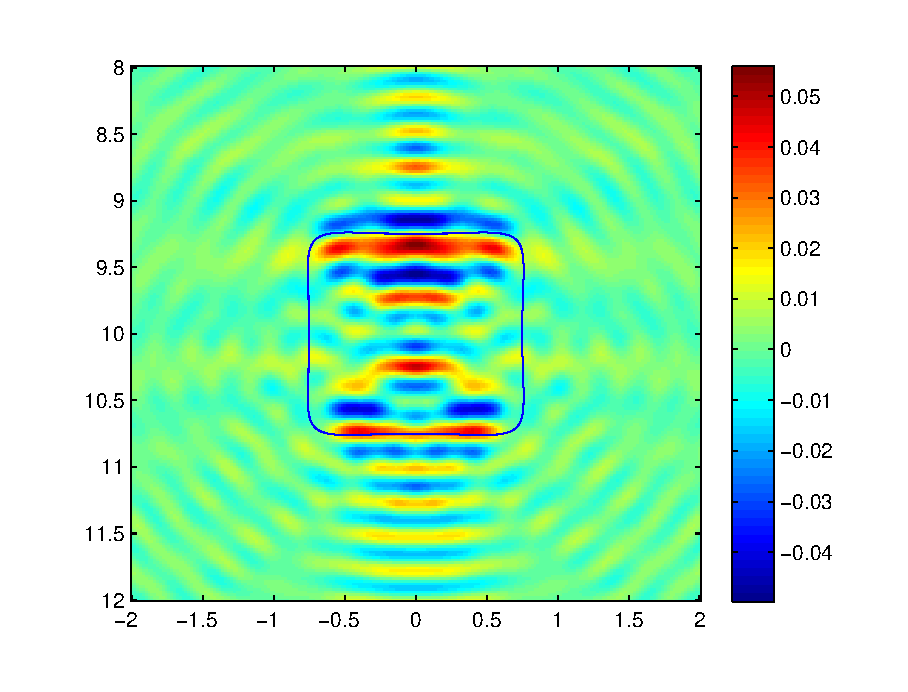
\includegraphics[width=0.23\textwidth]{./phaseless/ex1/ex1phaseless2}
  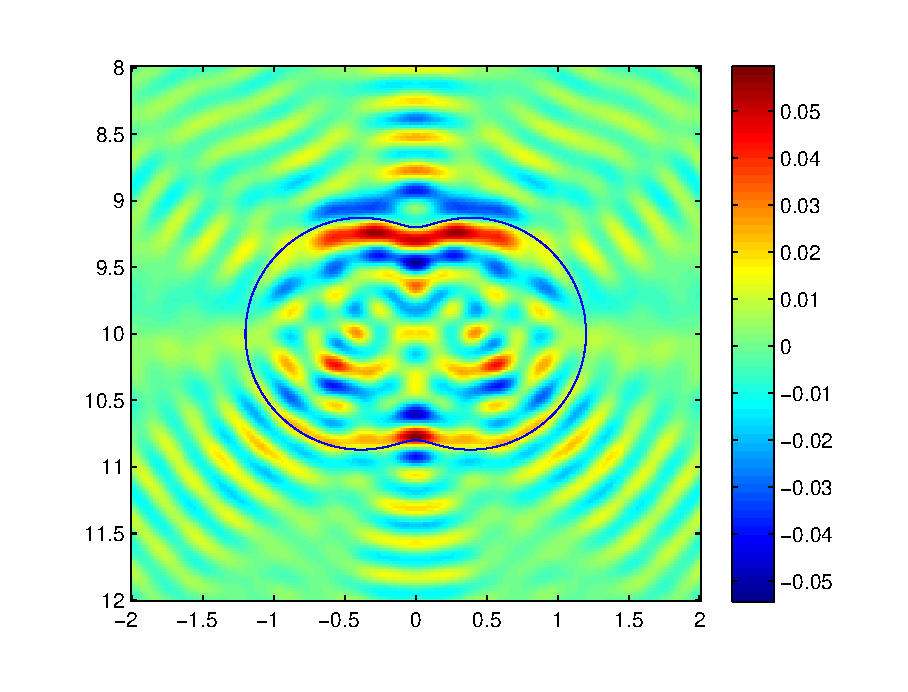
\includegraphics[width=0.23\textwidth]{./phaseless/ex1/ex1phaseless3}
  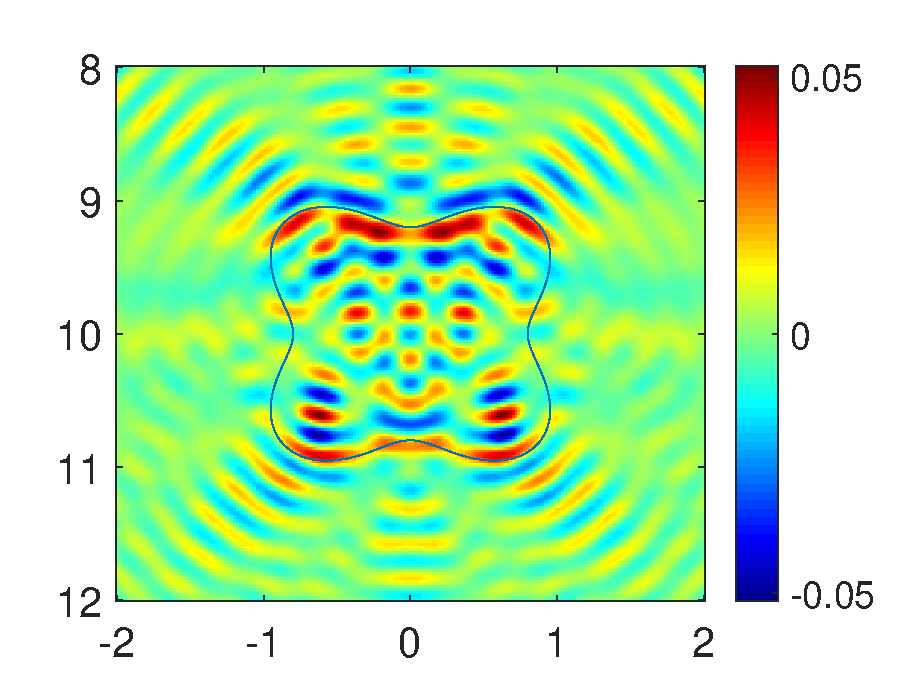
\includegraphics[width=0.23\textwidth]{./phaseless/ex1/ex1phaseless4}\\
  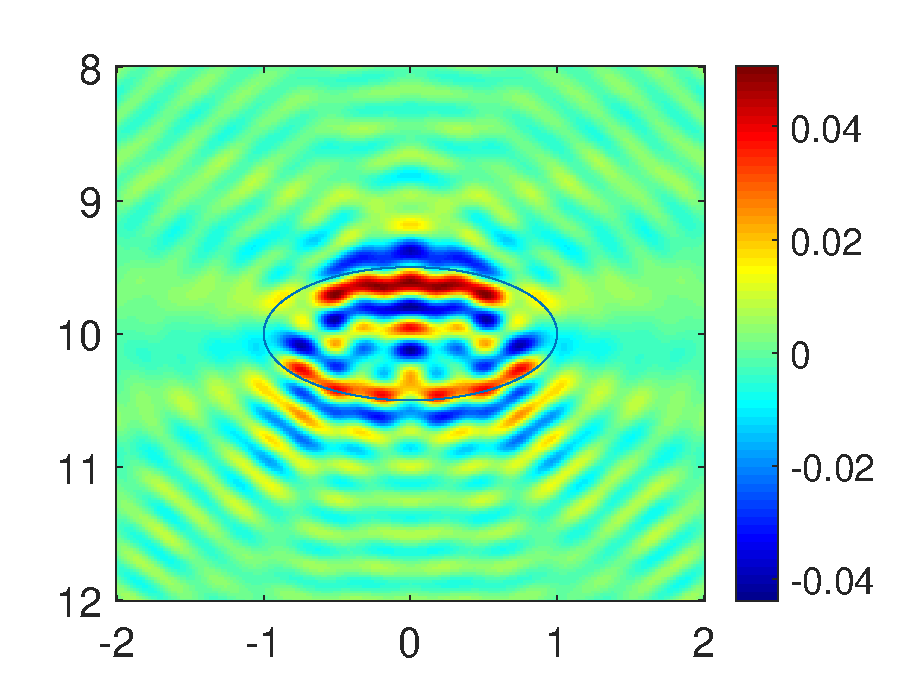
\includegraphics[width=0.23\textwidth]{./phaseless/ex1/ex1phase1}
  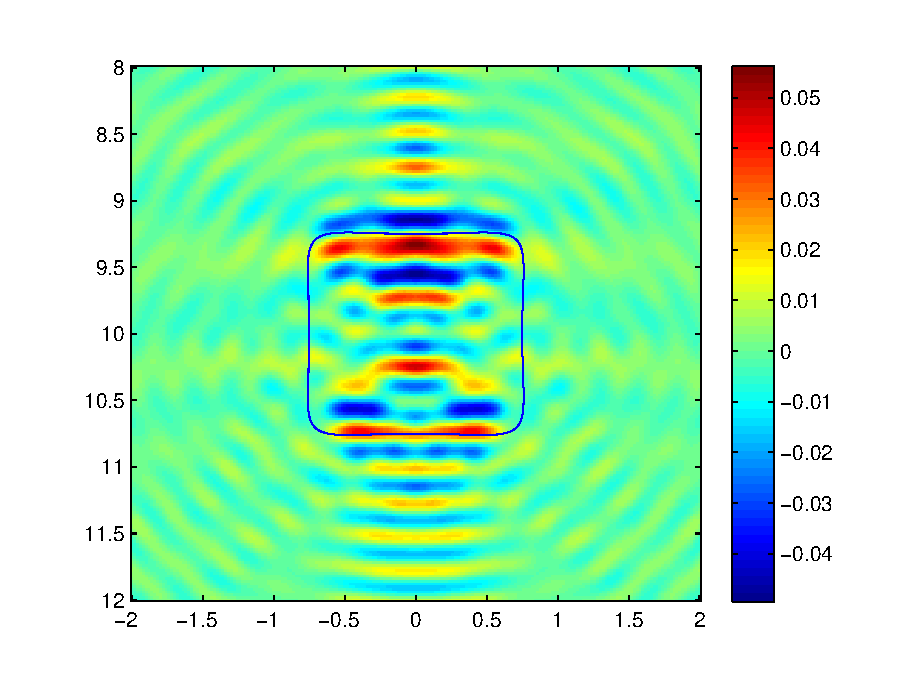
\includegraphics[width=0.23\textwidth]{./phaseless/ex1/ex1phase2}
  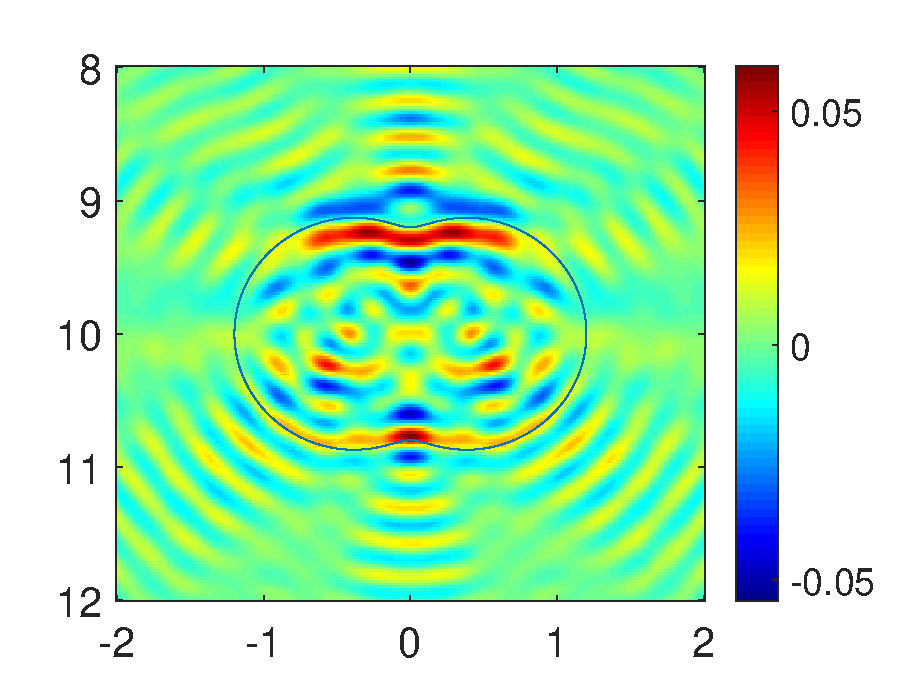
\includegraphics[width=0.23\textwidth]{./phaseless/ex1/ex1phase3}
  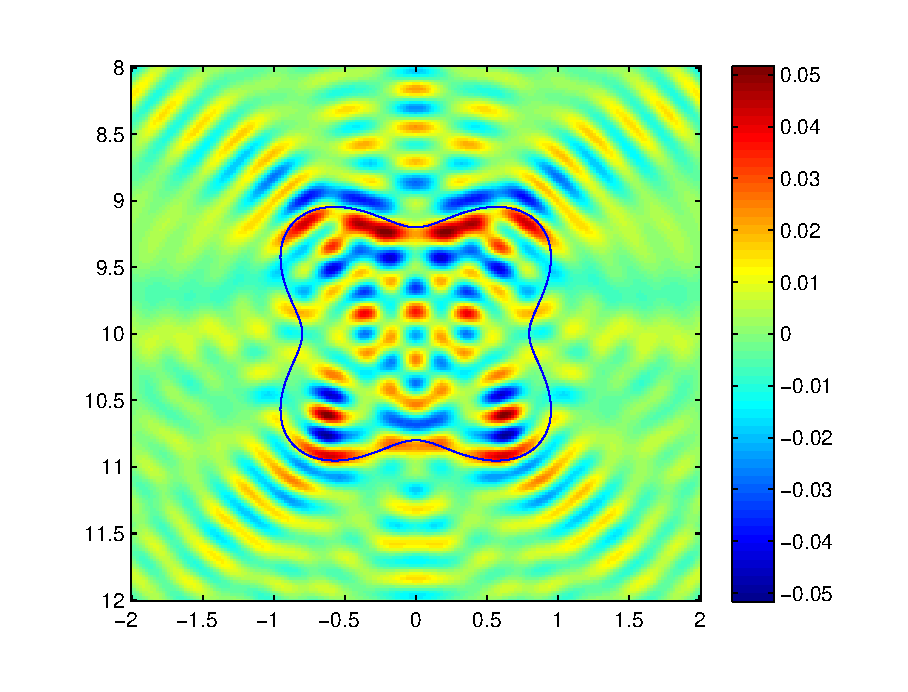
\includegraphics[width=0.23\textwidth]{./phaseless/ex1/ex1phase4}
  \caption{算例\ref{hp_ex1}:不同形状的可穿透障碍物,其中第一行为半空间无相位成像算法,第二行为半空间逆时偏移算法。参数为:$k=4\pi$, and $N_s=512$, $N_r=512$。} \label{fig1}
\end{figure}

\begin{example}\label{hp_ex2}
在本算例中,我们以具有椭圆形状的障碍物为例,考察新提出的半空间无相位逆时偏移算法对具有不同边界类型的障碍的成像效果,如声软障碍物,声硬障碍物以及阻尼系数为$\eta=1$的阻抗边界障碍物。采样区域为$\Omega=[-2,2]\times[8,12]$,且
我们使用$201\times201$的均匀采样。探测频率$k=4\pi$,源点和接收点个数为$N_s=512$, $N_r=512$。

图片 \ref{fig2}表明了仅仅使用总场的无相位数据,新算法也可以对各种边界类型的障碍物边界进行成像,确定其位置和形状。此外,我们强调一下,因为在$x_r\in\Gamma_0^d$接收到的数据并不包含障碍物下边界的信息,所以对不可穿透障碍物,仅能对障碍物上边界进行成像。
\end{example}
\begin{figure}[h]
  \centering
  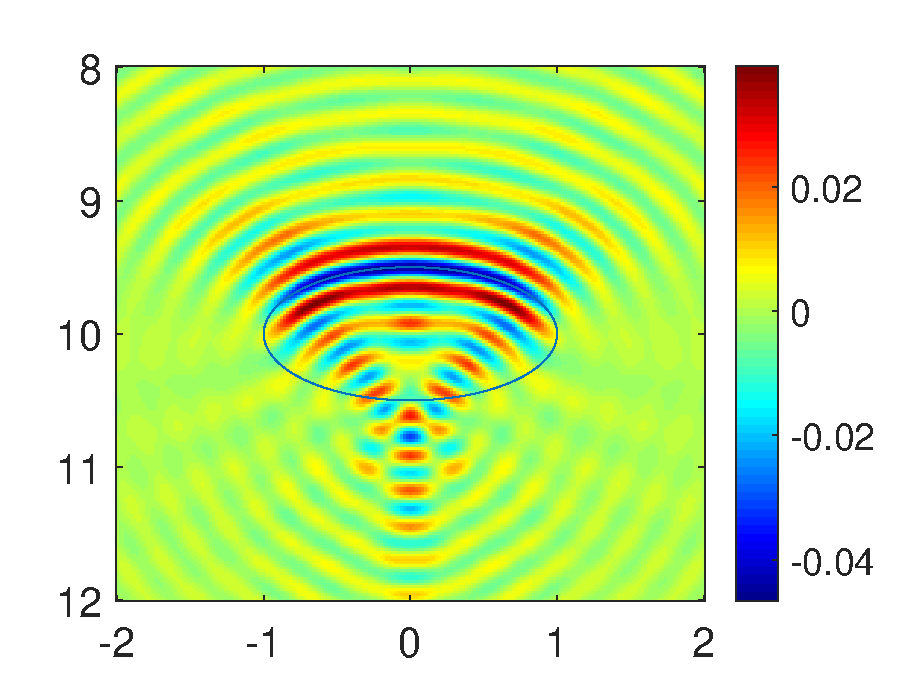
\includegraphics[width=0.3\textwidth]{./phaseless/ex2/ex2elliptic2}
  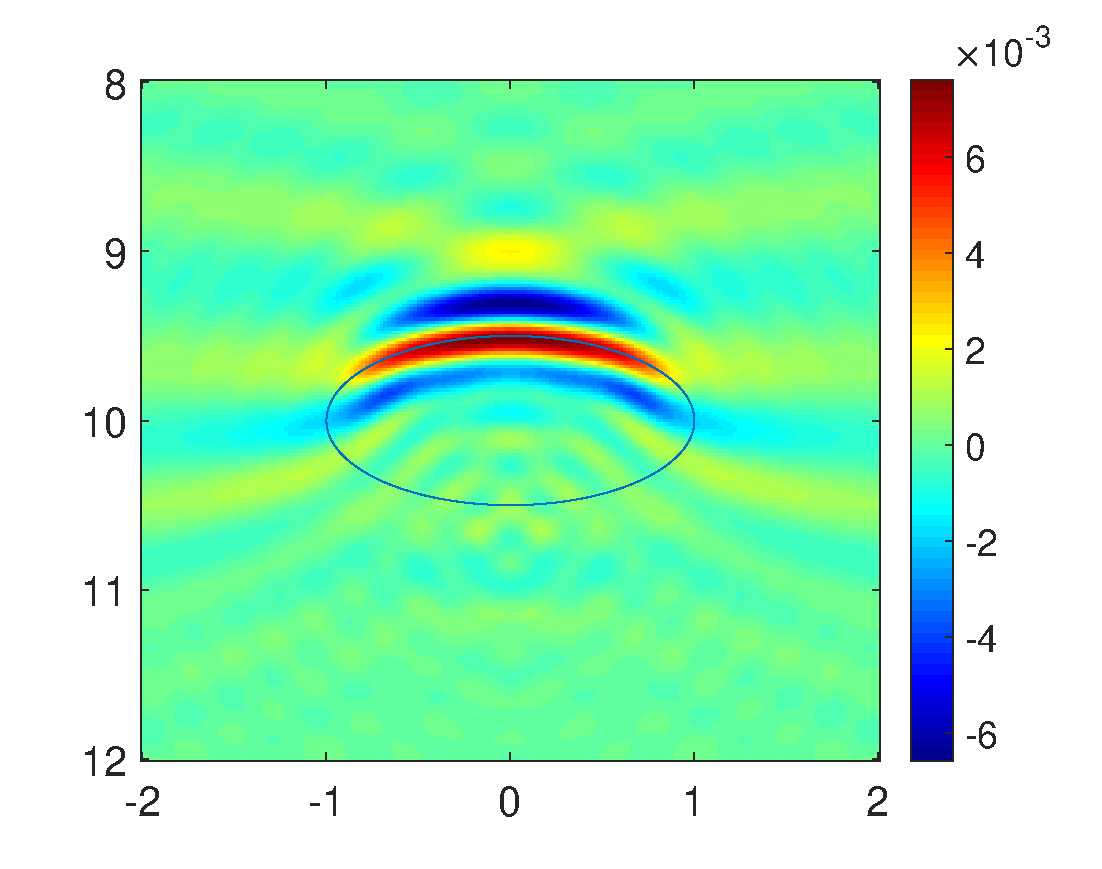
\includegraphics[width=0.3\textwidth]{./phaseless/ex2/ex2elliptic3}
  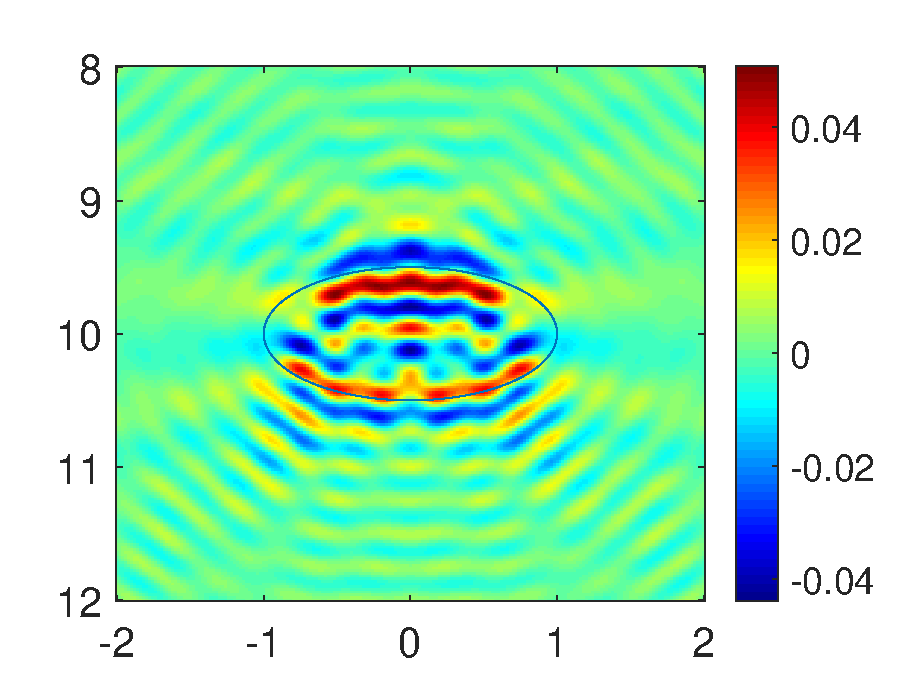
\includegraphics[width=0.3\textwidth]{./phaseless/ex2/ex2elliptic4}
    \caption{算例\ref{hp_ex2}:不同类型的椭圆型障碍物,从左到右依次为声软、声硬和阻抗系数为$\lambda\equiv1$的阻抗障碍物 。 参数为:$k=4\pi$, and $N_s=512$, $N_r=512$。}\label{fig2}
\end{figure}
\begin{example}\label{hp_ex3}
在本算例中,我们分别以单个频率和多个频率,来考察新提出的半空间无相位逆时偏移算法的抗干扰性。假设接受到的总场数据中带有如下形式的高斯噪音,
$$ |u|_{noise}=|u|+v_{noise},$$
其中
$$v_{noise}=\mu \max{|u|}\epsilon,\ \ and\ \ \epsilon\sim N(0,1).$$
采样区域为$\Omega=[-2,2]\times[8,12]$或者$\Omega=[-5,5]\times[6,16]$,且
我们使用$201\times201$的均匀采样。探测频率$k=4\pi$或$k=2\pi\times[1:0.25:3]$,源点和接收点个数为$N_s=256$, $N_r=256$。

在我们的第一个测试中,我们采用单个的可穿透障碍物作为成像目标,首先使用单频$k=2\pi$作为探测频率。图片 \ref{fig3}的第一行验证了当新算法使用带噪音的数据时,依然可以对障碍物进行有效成像,其中噪音水平依次为$\mu = 10\%, 20\%, 30\%, 40\%$。这就很好地验证了当噪音水平不断变大时,成像算法的稳定性。然后我们使用多频的数据来期望进一步提高成像效果,取频率为$k=2\pi\times[1:0.25:3]$。图片 \ref{fig3} 的第二行展示了相应噪音水平下多频的成像效果。可以看到,当采用多个频率时,噪音和振荡被抵消和压制,聚焦效果更加明显,极大地提升了成像效果。

在我们的第二个测试中,我们采用两个声软障碍物来作为成像目标,同样分别采用单频和多频以便加以对比。采样区域为$\Omega=[-5,5]\times[6,16]$,且我们使用$201\times201$的均匀采样。图片\ref{fig4}展示了不同噪音水平下,使用总场无相位数据时,新算法对多个障碍物的成像效果,同样我们观察到多频叠加的抗干扰能力和聚焦能力得到显著提高。在文献\cite{Robert2007Inverse}的定理4.1中,Robert Gilbert对Pekeris开波导模型下,证明了可穿透障碍物反散射问题的唯一性。
\end{example}

\begin{figure}[h]
  \centering
  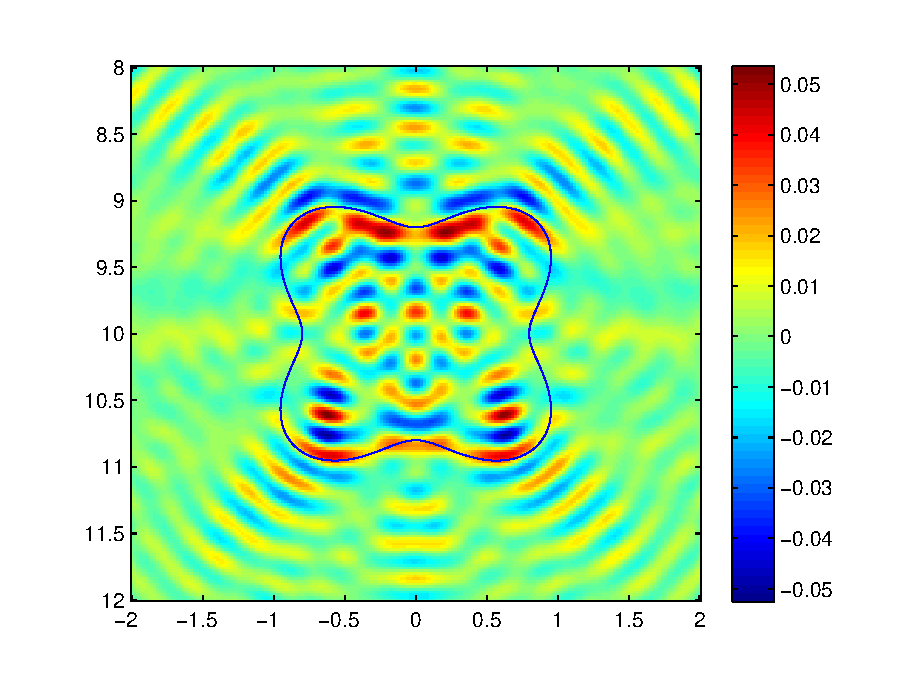
\includegraphics[width=0.23\textwidth]{./phaseless/ex3/ex3singlefreqsigma1}
  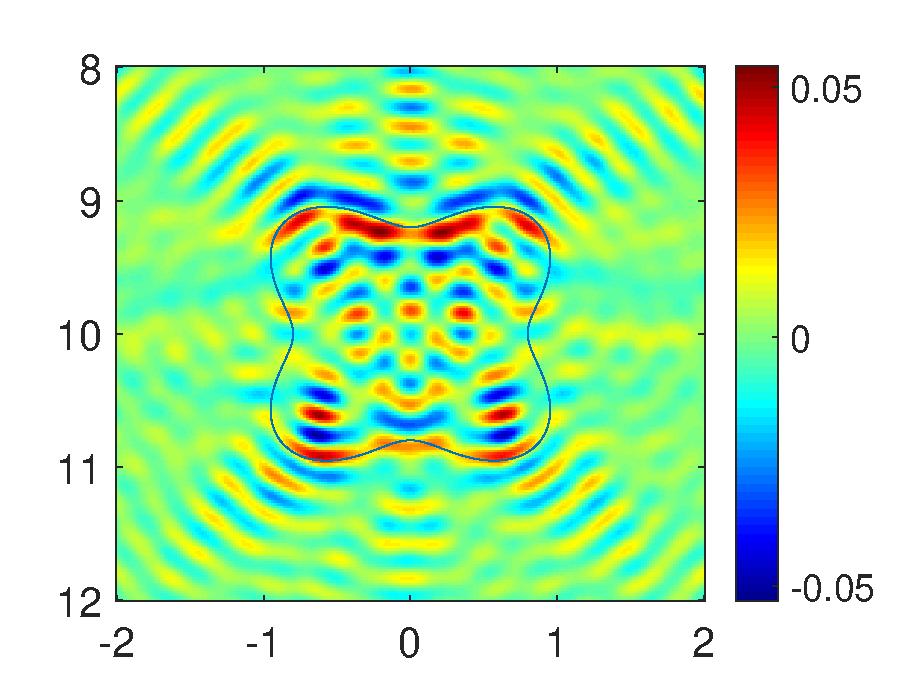
\includegraphics[width=0.23\textwidth]{./phaseless/ex3/ex3singlefreqsigma2}
  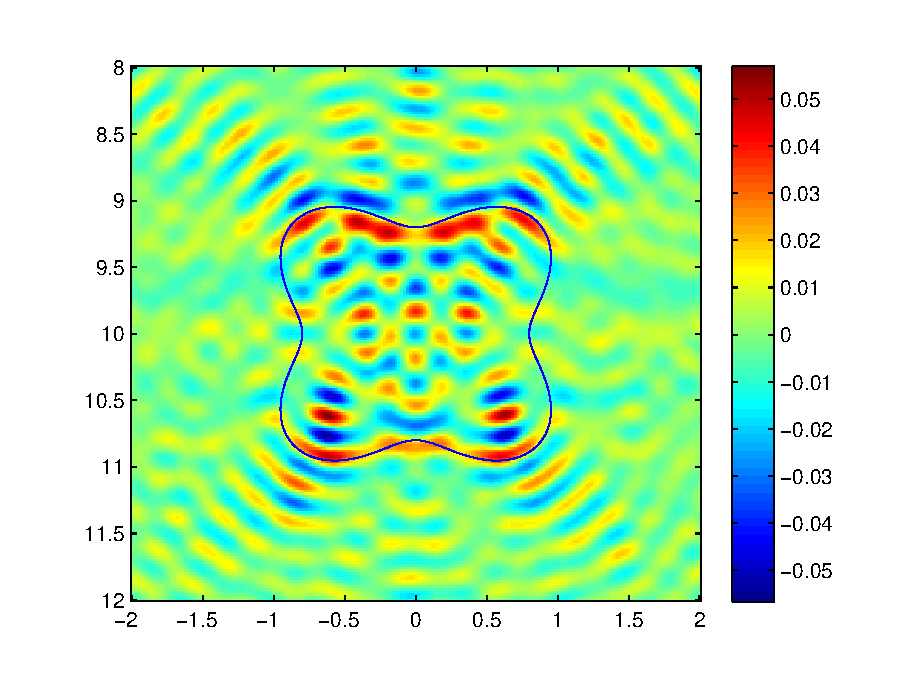
\includegraphics[width=0.23\textwidth]{./phaseless/ex3/ex3singlefreqsigma3}
  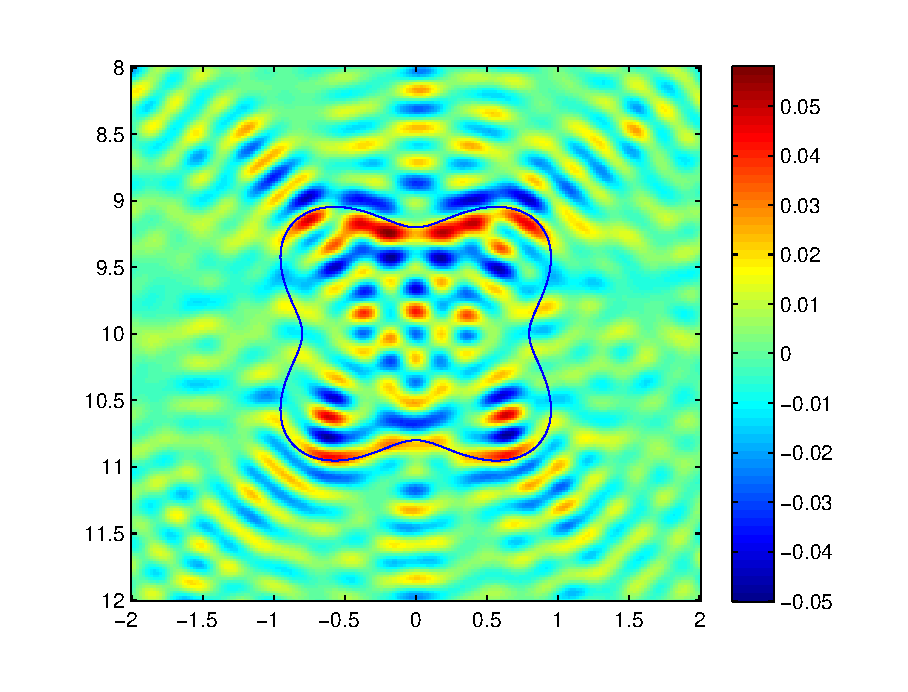
\includegraphics[width=0.23\textwidth]{./phaseless/ex3/ex3singlefreqsigma4}\\
  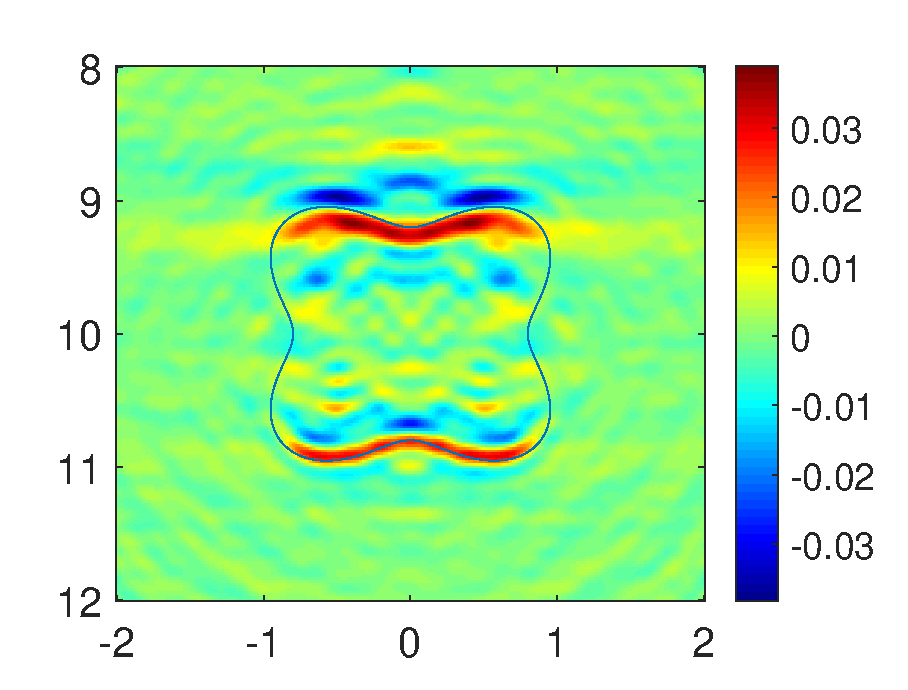
\includegraphics[width=0.23\textwidth]{./phaseless/ex3/ex3multifreqsigma1}
  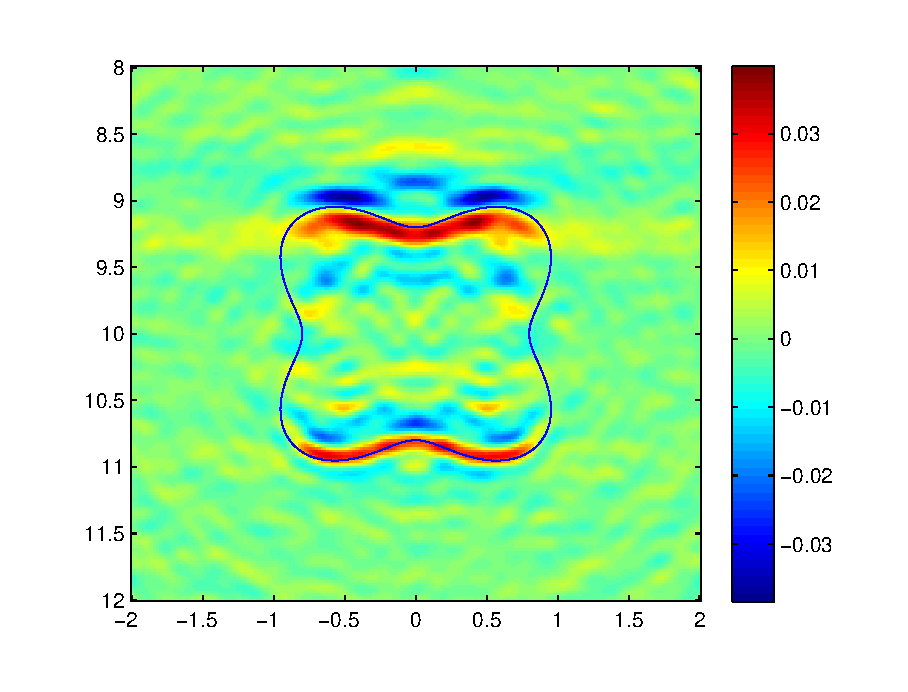
\includegraphics[width=0.23\textwidth]{./phaseless/ex3/ex3multifreqsigma2}
  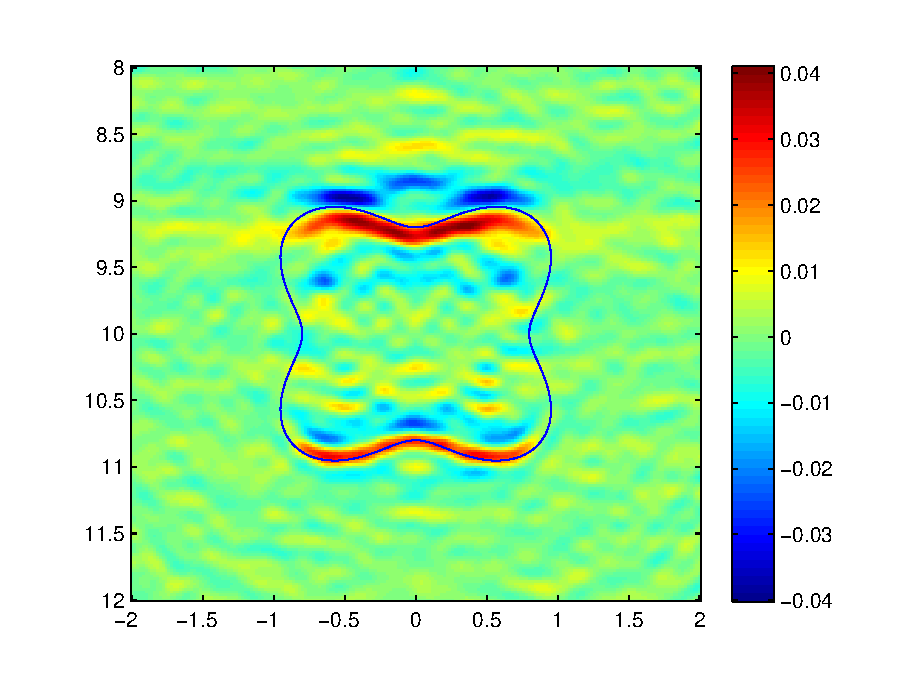
\includegraphics[width=0.23\textwidth]{./phaseless/ex3/ex3multifreqsigma3}
  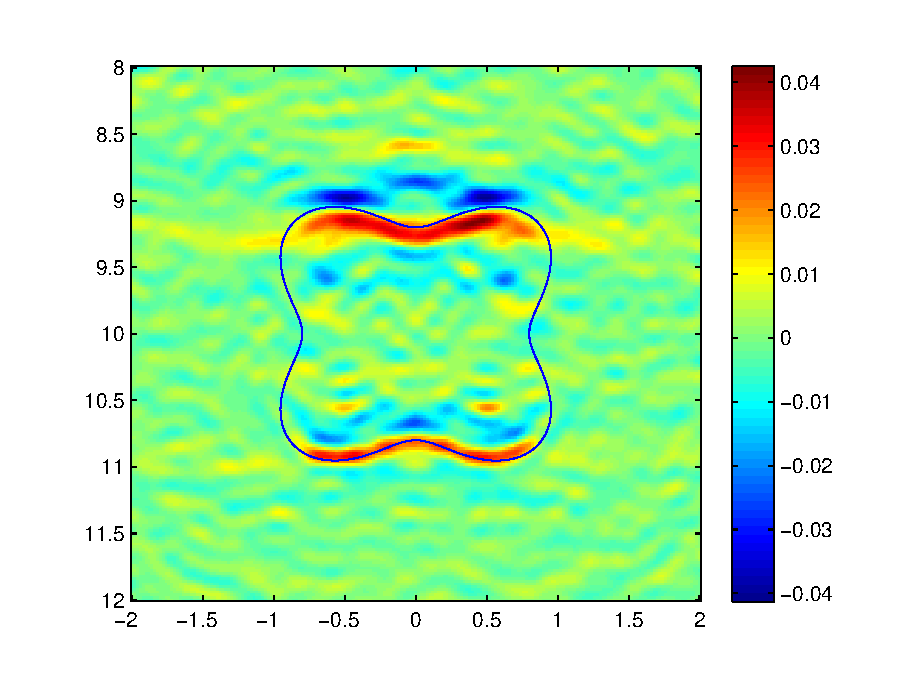
\includegraphics[width=0.23\textwidth]{./phaseless/ex3/ex3multifreqsigma4}
    \caption{算例\ref{hp_ex2}测试1: 带噪音数据的可穿透障碍物成像,噪音水平从左到右依次为为: $\mu=0.1,0.2,0.3,0.4$。
    第一行是单频测试结果,第二行为多频叠加结果。}\label{fig3}
\end{figure}
\begin{figure}[h]
  \centering
    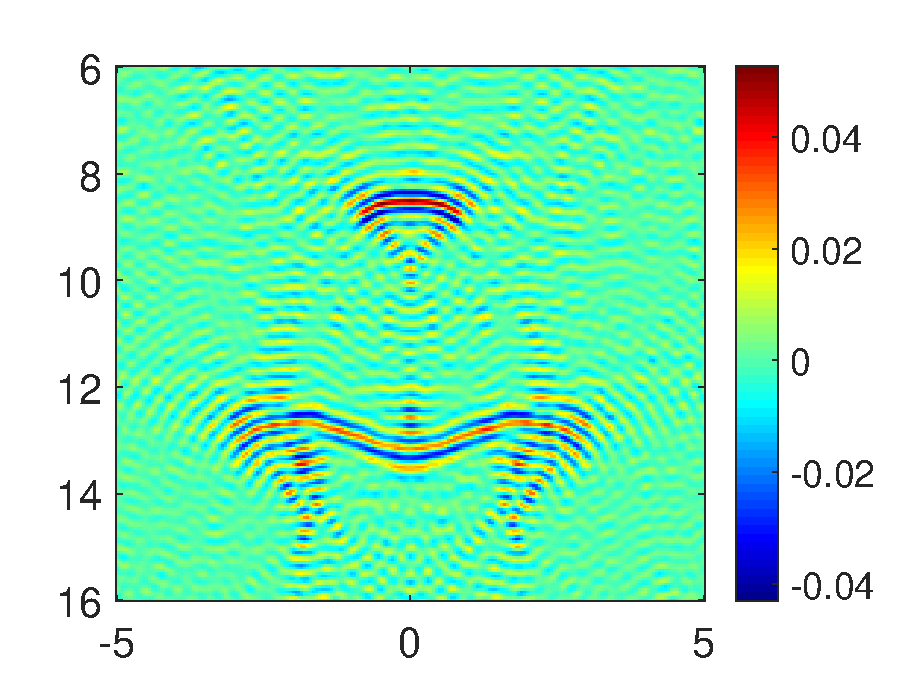
\includegraphics[width=0.23\textwidth]{./phaseless/ex4/ex4singlefreqsigma1}
  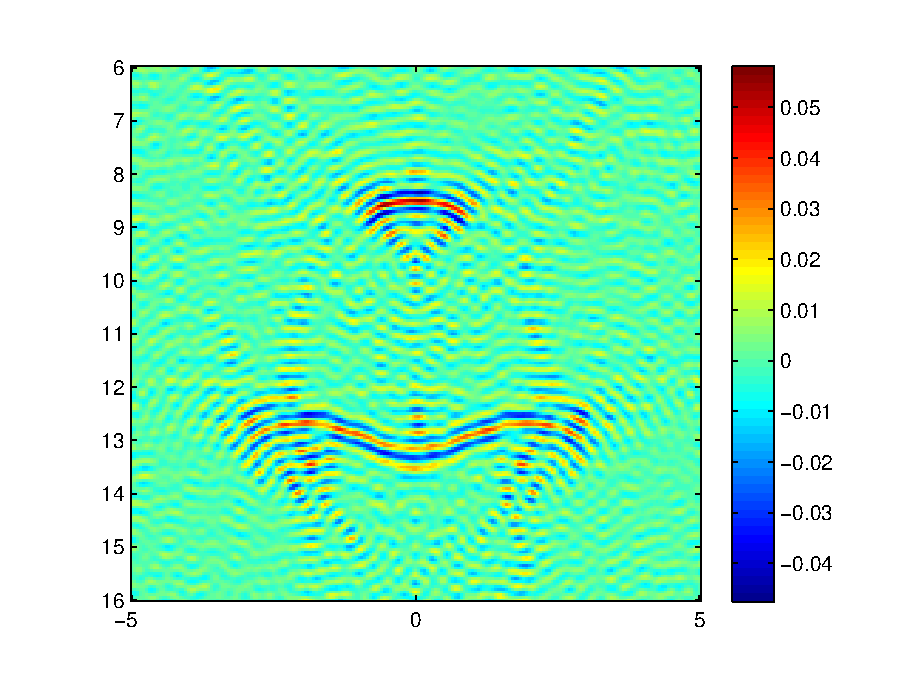
\includegraphics[width=0.23\textwidth]{./phaseless/ex4/ex4singlefreqsigma2}
  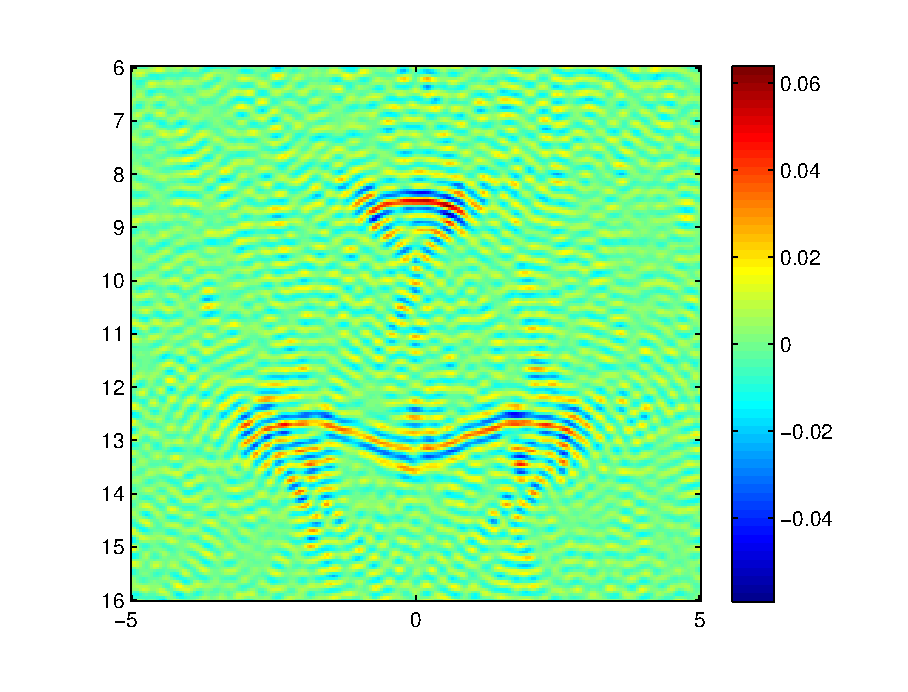
\includegraphics[width=0.23\textwidth]{./phaseless/ex4/ex4singlefreqsigma3}
  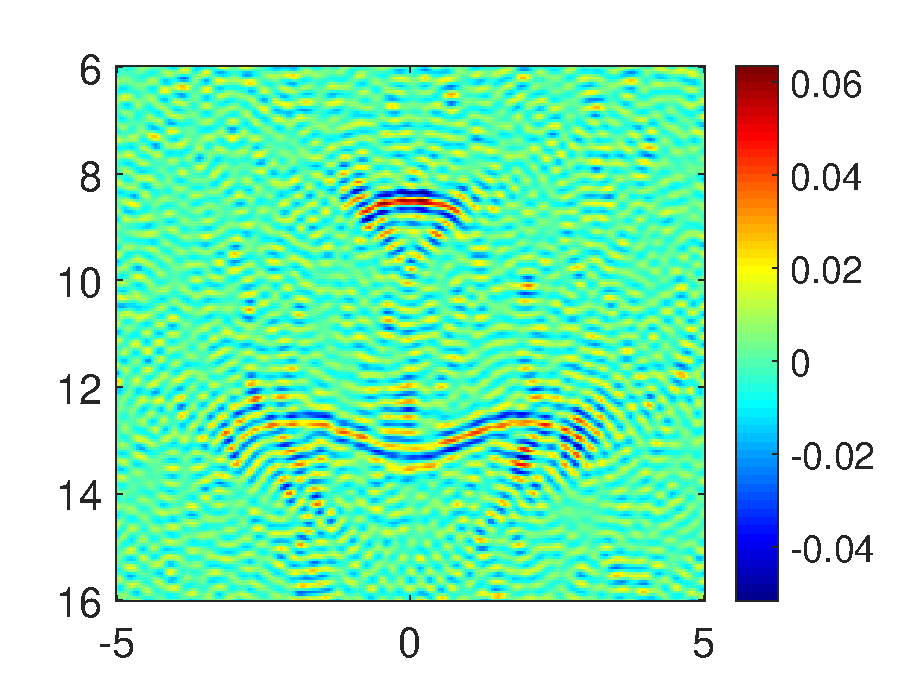
\includegraphics[width=0.23\textwidth]{./phaseless/ex4/ex4singlefreqsigma4}\\
      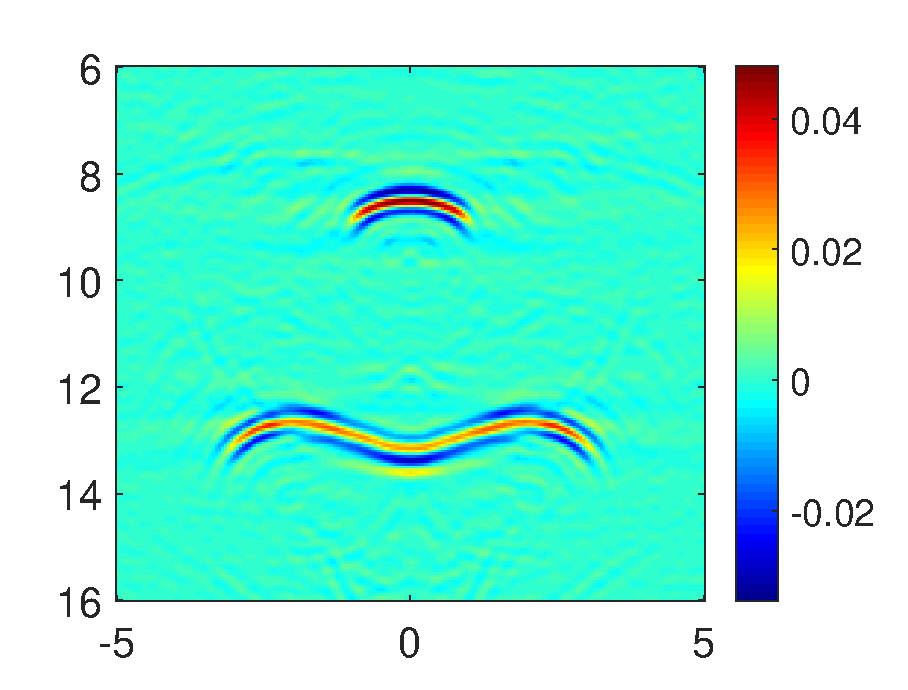
\includegraphics[width=0.23\textwidth]{./phaseless/ex4/ex4multifreqsigma1}
  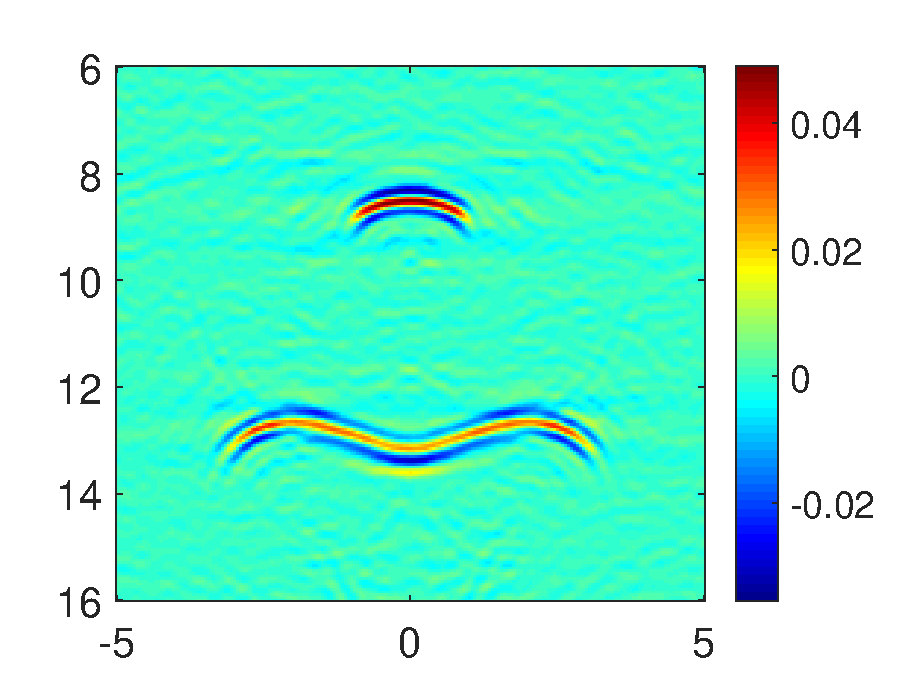
\includegraphics[width=0.23\textwidth]{./phaseless/ex4/ex4multifreqsigma2}
  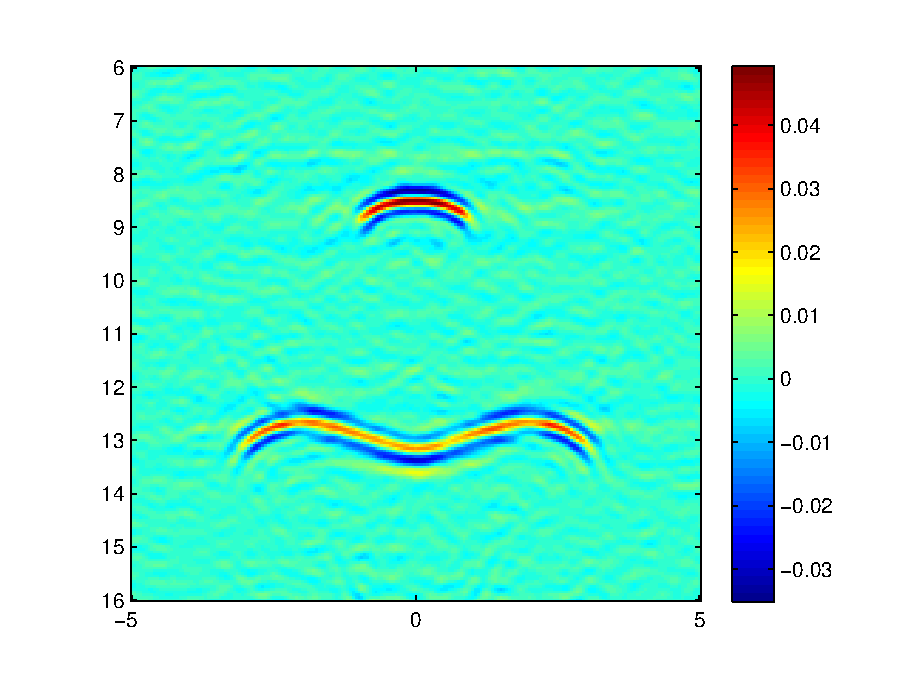
\includegraphics[width=0.23\textwidth]{./phaseless/ex4/ex4multifreqsigma3}
  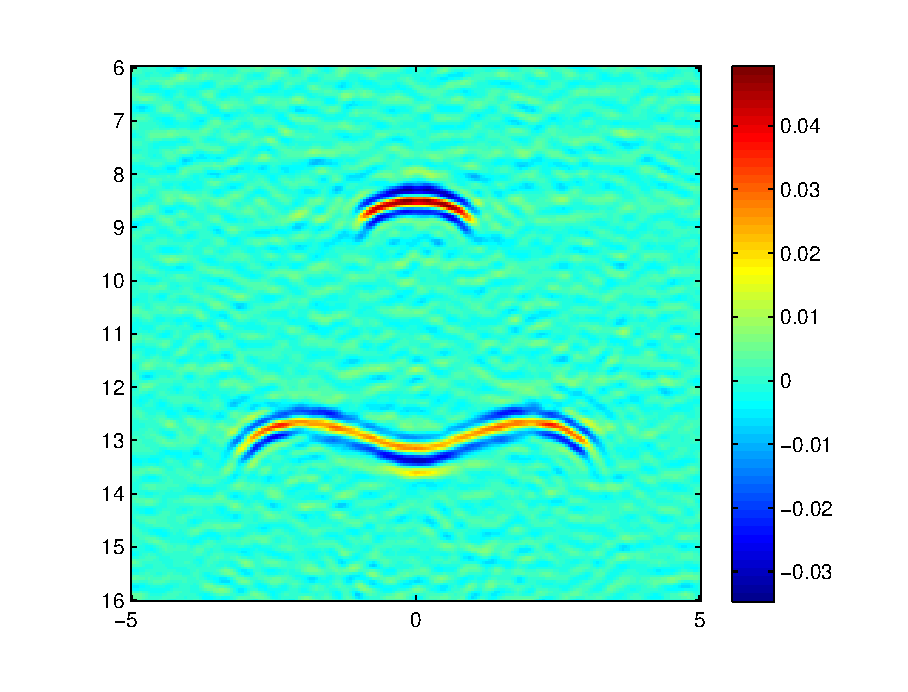
\includegraphics[width=0.23\textwidth]{./phaseless/ex4/ex4multifreqsigma4}
    \caption{算例\ref{hp_ex2}测试2: 带噪音数据的两个声软障碍物成像, 参数设置与\ref{fig3}完全一样。}\label{fig4}
\end{figure}
\begin{remark}
从上一节的数值测试结果可以看出,在障碍物$D$远离半空间边界$\Gamma_0$时,本章所提直接成像算法\ref{alg_phaseless}可以达到文献\cite{ch_ha}中所提半空间逆时偏移算法相同的分辨率。同样的,对于不可穿透障碍物,算法\ref{alg_phaseless}仅能够对障碍物$D$上半边界进行成像。这种现象在文献\cite{ch_ha}通过高频渐进分析和散射系数进行了说明,为了保证完整性,我们将在本文附录对Hemholtz散射系数加以补充和说明,此处不再详述。
\end{remark}
\section{本章小结}

在本章,我们主要考虑了声波半空间障碍物成像问题。特别地,我们提出了一种直接成像算法\ref{alg_phaseless}。该算法可以解决如下问题:

当在半空间边界$\Gamma_0:=\{(x_1,x_2)\in\R^2_+,x_1\in\R,x_2=0\}$上所采集的数据为无相位数据$u(x_r,x_s)$时,如何快速高效确定障碍物的位置、大小和形状?

除此之外,我们还对算法\ref{alg_phaseless}进行了分辨率分析,理论研究表明:当障碍物$D$远离半空间边界$\Gamma_0$时,算法\ref{alg_phaseless}可以达到文献\cite{ch_ha}中半空间逆时偏移算法相同的分辨率。数值测试表明算法\ref{alg_phaseless}还继承了半空间逆时偏移算法的优点:在不需要知道障碍物的任何信息的情况下,例如是否可穿透以及可穿透障碍物的边界条件,算法\ref{alg_phaseless}能够对不同类型不同形状的障碍物进行有效成像;并且算法的抗噪性能和多频测试结果也都令人十分满意。